% @Date:   2019-04-01 23:02:29
% @Last Modified by:   Discount

\documentclass[UTF8]{article}
    \author {刘林冬、齐向彤、徐宙}
    \title {基于拉格朗日松弛理论的非平衡博弈
费用分摊算法}
    \date{}
\usepackage{ctex}
\usepackage{amsmath}

\usepackage{geometry}
\geometry{a4paper,scale=0.8}
\usepackage{graphicx}
\usepackage{amssymb}

\usepackage{setspace}
\renewcommand{\baselinestretch}{1.5}

\usepackage{natbib}
 \bibpunct[, ]{(}{)}{,}{a}{}{,}%
 \def\bibfont{\small}%
 \def\bibsep{\smallskipamount}%
 \def\bibhang{24pt}%
 \def\newblock{\ }%
 \def\BIBand{and}%

 \usepackage{float}
 \usepackage{color}%,soul}f
 \usepackage{multirow}
 \usepackage{xr}
 \externaldocument{online-supplement}

 \newtheorem{algorithm}{Algorithm}
 \newtheorem{pf}{Proof}
 \newcommand*{\QEDB}{\hfill\ensuremath{\square}}

 \newcommand{\rv}{random variable}
 \newcommand{\bE}{\bf E}
 \renewcommand{\Box}{\bigboxvoid}
 \newcommand{\qeds}{$\qedsymbol $}
 \newcommand{\R}{\mathbb{R}}
 \newcommand{\Z}{\mathbb{Z}}
 \newcommand{\cc}{\mathbb{c}}

\begin{document}
    \maketitle
\begin{abstract}
针对核为空的合作博弈费用分摊问题,本文研究了在满足大联盟稳定条件下将分摊给所有参与者的总费用最大化的算法。此类问题的应用之一就是找到稳定大联盟所需的最低补贴费用。为求解此问题,我们提出了基于拉格朗日松弛理论的非平衡博弈费用分摊算法。与现有的基于线性松弛理论的算法相比,本文提出的算法可以得到更好结果,并且其适用范围也更加广泛。为证明该算法的有效性,本文研究了两种不同的设施选址博弈。结果表明,该算法不仅保证了新算法的效用,而且很大程度的拓展深化了费用分摊问题的研究广度与深度。

\end{abstract}
\qquad \textbf{关键词: 博弈论、合作博弈、费用分摊、拉格朗日松弛、设施选址博弈}

\section{引言}
合作博弈理论解决了多个独立决策人之间的合作问题。它在经济、金融、运筹学(OR)和电信等多个领域都有应用。在降低成本的问题中, (具有可转移效用的) 合作博弈可以大致表述为:有$n$个参与者,每个参与者都需要利用其资源以最小的费用完成既定的任务目标。为了降低总成本,有些(或所有)参与者可能会通过结盟的方式集中资源实现任务目标。所有参与者的集合被称为大联盟。主要的问题是如何以“公平”的方式分摊大联盟的费用,使得任何一位参与者不会退出。
定义费用分摊的“公平”有不同的方法,但是一个根本的概念就是联盟的稳定性。保证联盟的稳定性需满足分摊给每个联盟的成本 (分摊给联盟中每个参与者的成本之和)不超过联盟成员未加入联盟时的最低成本。另外,为保证公平,还需满足分摊给所有参与者的总成本等于大联盟最低成本的预算平衡约束。合作博弈的核心是联盟的费用分配集满足(1)联盟稳定性和(2)预算平衡约束。如果至少存在一个这样的分配,那该博弈的核心就不为空,大联盟就是稳定的。目前已有许多方法可以判断各种合作博弈的核是否为空。
然而许多合作博弈问题都是空核。对于空核博弈,已经有人提出了用替换的概念来给出解决方案。其基本思想是松弛核心定义的两个条件之一。例如,松弛联盟稳定性的最小核概念{\em least core} (e.g., \citealt{maschler1979geometric,Kern2003,Uhan2010,Uhan2013LeastCore})。在最小核概念中,分摊给每个联盟的费用不超过$z$与联盟的最小成本之和,其中z是一个最小化的参数。
在另一个被称为{\em $\gamma$-核}(e.g., \citealt{Jain2007CostSharing})的概念中,预算平衡约束被替换为$\gamma$预算平衡约束。$\gamma$预算平衡约束指分摊给所有参与者的总成本不小于$\gamma$乘以大联盟的最低费用,其中$0<\gamma\leq 1$。在数学领域{\em $\gamma$-核}等同于另一个概念{\em $\epsilon$-近似核}(e.g., \citealt{Faigle1998EuclideanTSPGamesCore,Blaser2008MetricTSPGamesCore})。这一概念约束预算平衡,松弛联盟稳定性,使分配给每个联盟的成本之和不超过$(1+\epsilon)$倍的联盟的最低费用。总之,研究$\gamma$-核 或 $\epsilon$-近似核的关键点是在具体的博弈中找到$\gamma$或$\epsilon$的连续边界。
在本文中,我们探究了$\gamma$-核。但与原文的关注点不同,对于由Caprara和Letchford提出的最优费用分摊问题(OCAP),我们设计了一种算法来精确计算任意给定博弈的最佳$\gamma$值,而不是只寻找$\gamma$的连续边界。特别地,OCAP问题尝试最大化分摊给所有参与者的总费用\cite{Caprara2010LPB},这可以等价地看作计算大联合政府为保持社会稳定最优状态的“费用”。在大联合政府中,代表社会福利的第三方愿意为大联合政府的稳定提供补助。在这里,第三方可能是政府机构,而参与者是一群私营公司。或者,第三方是一个大公司的总部,而参与者是不同的分公司。在这种情况下,OCAP的目标相当于最小化分配给所有参与者的总费用与大联盟总费用之间的差值,而这一差值则由第三方提供补助。
简单地说,找到OCAP的解至少有两个困难。首先,普通线性规划(LP)公式的约束数量随着参与者数量的增加而指数级增加,即$n$个参与者需要$2^n$个约束。其次,对于给定的费用分摊方案,仅验证其中一个LP约束是否被满足,就需要解NP-hard的优化问题。因此,直接用LP公式求解OCAP是非常困难的。
对于空核的合作博弈问题,首先想到的就是求解OCAP。然而,该问题一直未得到充分的研究,直到\cite{Caprara2010LPB}提出了一个基于线性松弛理论的算法(LPB算法)。其基本思想是建立一个稳定的费用分摊方法。该方法可以得到大联盟成本的线性松弛下界。从理论上讲,LPB算法是可以最好地解决OCAP,但前提是识别并添加ILP公式中的所有“可分配”约束。然而,有时很难识别所有可分配的约束。如果没有多项式时间间隔算法来处理可分配约束的指数数量,即使在所有可分配的约束都可以被识别的情况下,LPB算法仍然是不适用的。例如,研究的无根旅行商博弈。
本文基于拉格朗日松弛理论,提出了一个的新算法处理OCAP。该方法(LRB算法)虽然也试图找一种费用分摊方案使大联盟费用达到更低,但与LPB算法相比具有以下优势。
首先,它是一个通用算法,可以应用于比
\cite{Caprara2010LPB}所描述的更广泛的合作博弈。而且与LPB算法只能解决线性目标函数不同,新算法也适用于具有非线性目标函数的问题。
其次,由于拉格朗日松弛界不比松弛LP解提供的界差,对于模型相同的大联盟问题LRB算法可以找到比LPB算法更好的解。在一定程度上,这避免了LPB算法中识别所有“可分配”约束的要求。此外,即使在某些可找到所有可分配约束情况下,LRB算法仍然是有价值的。因为它可以为参与者提供可替代的最优费用分摊方案,从而提供更多的评估选择。
第三,在求解OCAP时,LRB算法利用分解的方法将原博弈问题分解为两个子博弈。子博弈1可以得到用闭型表示的最优解。子博弈2可以具有一些原博弈所缺的特性。在许多情况下与原博弈相比,子博弈中每个联盟产生的最小费用更容易计算。在某些情况下,子博弈的最优成本分配是多项式可解的,而原始博弈的最优成本分配不是多项式可解的。
最后,LRB算法是依赖于几十年来求解拉格朗日对偶问题的大量研究。在将它应用到OCAP时,我们可以充分利用各种加速收敛和生成更清晰界限的方法。这些结果可以在LRB算法的第一步中进行合并。

\section{文献综述}\label{sec:review}
自\cite{shapley1952value}的开创性工作以来,合作博弈的研究一直在深入研究。与运筹学应用相关的领域最为突出,主要包括分配博弈(\citealt{Shapley1971AssignmentGame,Martinez2013})、装箱博弈(\citealt{Faigle1993,Liu2009})、线性生产博弈(\citealt{Owen1975LinearProductionGames})、最小生成树博弈(\citealt{Granot1981MinimumSpanningTreeGames})、旅行商博弈(\citealt{Tamir1989TSPGames,Potters1992})、车辆路径规划博弈(\citealt{Gothe1996VehicleRoutingGames,Engevall2004})、库存博弈(\citealt{Hartman2000, Chen2009, Chen2009b, He2012,Zhang2009})、生产外包博弈(\citealt{Aydinliyim2010,Cai2012})以及一些图形包装和覆盖博弈(\citealt{Deng1999PackingAndCoveringGames})等。这些博弈的研究重点通常是核心的存在性。
本文以设施选址博弈为例。\cite{Kolen1983FacilityLocationGame}给出了一个早期的重要结果。他指出,对于无容量设施选址(UFL)博弈,参与者的最大分摊费用等于大联盟优化问题的经典LP松弛成本。后来,\cite{Goemans2000FacilityLocationGames}在此基础上扩展了这一研究,并证明了在一些特殊的设施选址博弈中的核心非空,如地址在一条线上、一个循环和一个树形网络上。其他人也研究了这个问题的变形。如\cite{Puerto2011,Puerto2012}分别介绍了最小半径选址博弈和最小直径选址博弈。\cite{Xu2009}, \cite{Mallozzi2011},\cite{Li2012UFLPConcave}等人研究了考虑各种成本要素的设施定位博弈,如服务安装成本,区域固定成本,以及凹形设施选址成本。
如前文所述,最小核是一种可用于处理空核博弈的松弛方法。\cite{faigle2000note}指出,计算最小生成树博弈的最小核分配是NP-hard问题。\cite{Kern2003}基于基数匹配博弈中最小核的多项式描述研究了核仁。\cite{Uhan2010}的研究表明求一个具有超模成本单机调度博弈的最小核值是弱NP-hard问题,并为计算最小核值的3-approximate算法(界为3)提供了方法\cite{Uhan2013LeastCore}。关于$\gamma$-core 和 $\epsilon$-approximate core,使用后者进行研究的更多。例如,\cite{Faigle1998EuclideanTSPGamesCore}提出了一种基于LP的算法,为Euclidean TSP博弈得出了一个 $\frac{1}{3}$ -近似核。\cite{Blaser2008MetricTSPGamesCore}提出了一种多项式时间算法,该算法可以在一个$(\log_2(n-1)-1)$ -近似核中得到非对称TSP博弈的费用分摊方法。我们建议读者参考 \cite{Jain2007CostSharing}的研究以对先前的概念进行更全面的回顾。
现在仅有几篇论文直接研究OCAP。\cite{Bachrach2009Cost}提出了在稳定合作博弈中大联盟的前提下,如何确定补贴的最小值并且得到最小值合适的上、下界的问题之后,\cite{Meir2011subsidies}进行了类似的关于联合博弈中限制合作的研究。目前唯一解决OCAP的算法是由\cite{Caprara2010LPB}提出的。他们提出了一种基于LP松弛和对偶理论的算法。在他们的方法中,通常需要通过引入具有特殊结构的约束来重新表达优化问题。详细内容将在下一节中介绍。

\section{正文前述}\label{sec:definition}
可转移效用的合作博弈用二元向量$(V,c)$表示,其中$V = \{1,2,...,v\}$表示参与者集合,$c:S \rightarrow \mathbb{R}$表示特征函数,$S= 2^V \setminus \emptyset$ 表示参与者非空的联盟集合。特征函数为每个联盟$s\in S$分配了一个值$c(s)$,代表了$s$中的成员在合作时需要支付的最小总成本。本文研究的费用分摊问题是在$V$中的参与者之间分摊大联盟的成本$c(V)$使得任何一个小联盟的参与者都没有动机脱离大联盟。
一个博弈$(V,c)$的稳定费用分摊是一个向量$\alpha \in \R^{v}$,其满足联盟稳定性:$\sum_{k \in s} \alpha(k) \leq c(s),~ \forall s \in S$。理想中的费用分摊另外满足预算平衡约束:$\sum_{k \in V} \alpha(k) = c( V)$ 。博弈$(V,c)$的核心定义为:
\begin {equation*} \label{eqn:budgetbalance}
Core(V,c)=\{\alpha \in \R^{v}:\sum_{k \in s} \alpha(k) \leq c(s),\forall s \in S, \mbox{ and } \sum_{k \in V} \alpha(k) = c( V)\}.
\end {equation*}
众所周知,并不是每个博弈$(V,c)$都有非空的核心。要求解核心为空的博弈,我们的目标是找到一个稳定的费用分摊方案,尽可能多地接近大联盟成本$c(V)$。这就是最优费用分摊问题,定义如下:
\begin{eqnarray}\label{eqn:OCAP}
\begin{aligned}
\begin{split}
\max_{\alpha} \sum_{k \in V} \alpha(k)&\\
s.t. \sum_{k \in s} \alpha(k) \leq  c(s),~ \forall &s \in S.
\end{split}
\end{aligned}
\end{eqnarray}
通常很难直接求解$(\ref{eqn:OCAP})$,因为它包含一个指数级的约束条件,而且计算特征函数$c(s)$可能是NP -难问题。本文的重点是为OR博弈求得稳定的最优费用分摊方案。该类博弈的核心可能为空,特征函数由整数规划定义,是\cite{Caprara2010LPB}研究的整数最小化(IM)博弈的推广。与只能使用ILP来定义特征函数的IM博弈不同,OR博弈允许使用非线性整数规划来定义特征函数。

\begin{definition}\label{def2}
如果一个博弈$(V,c)$满足以下条件,则该博弈被称为OR博弈。\\
$~~\bullet$
正整数 $r$, $r'$ 和 $t$,\\
$~~\bullet$ 左边矩阵 $A \in \R^{r \times t}$ 和 $A' \in \R^{r' \times t}$,\\
$~~\bullet$ 右边矩阵 $B \in \R^{r \times v}$和 $B' \in \R^{r' \times v}$,\\
$~~\bullet$ 右边非负列向量 $D \in \R^{r}$ and $D' \in \R^{r'}$,\\
$~~\bullet$ 线性或非线性目标函数 $f(x)$,\\
$~~\bullet$ 对于所有$s \in S$,示性列向量 $\gamma^s \in \{0,1\}^v$满足:若 $k \in s$且 $\gamma_k^s=0$, 则 $\gamma_k^s=1$ 否则, $\forall k \in V$,\\
则特征函数$c(s)$用整数规划表示为:
\begin{equation}\label{eqn:orgc}
c(s) = \min_{x} \big\{ f(x):Ax \geq B\gamma^s + D, A'x \geq B'\gamma^s + D', x \in \{0,1\}^{t \times 1} \big\}.
\end{equation}
\end{definition}

注意,在式$(\ref{eqn:orgc})$中,为方便使用拉格朗日松弛,约束被分为两部分。根据\cite{Caprara2010LPB}的研究,很容易证明每个OR博弈的非负列向量$D$和$D'$都具有次可加性,即对于任意 $s_1,s_2 \in S$ ,$c(s_1 \cup s_2) \leq c(s_1) + c(s_2)$, 且 $s_1 \cap s_2 = \emptyset$。
IM博弈是OR博弈的一种特殊类型,它的特征函数$c(s) $是由整数线性规划表示为:
\begin{equation}\label{eqn:orgc1}
c(s) = \min_{x} \big\{ Cx:Ax \geq B\gamma^s + D, A'x \geq B'\gamma^s + D', x \in \{0,1\}^{t \times 1} \big\},
\end{equation}
其中$C$是$t$维行向量.我们用$c_{LP}(V)$ 表示(\ref{eqn:orgc1})中$c(V)$的LP下界,其中$x \in \{0,1\}^{t \times 1}$ 松弛为 ${\bf 0}\leq x \leq {\bf 1}$。
\cite{Caprara2010LPB}给出了通过使用列生成、行生成或二者结合解决IM博弈的OCAP方法。,我们在online supplement中总结了这些方法的要点。列生成方法有一个简单的公式,但由于优化过程中需要极大的解空间,与其相关的定价问题通常很难处理。行生成方法需要通过识别被称为可分配约束的集合$\{ Ex \geq F\gamma\}$来重新确定ILP(\ref{eqn:orgc1})。然后,通过求解仅具有可分配约束的LP松弛$c_{LP}^{EF}(V)=\min\{ Cx : Ex \geq F\gamma\}$得到费用分摊方案,其中总费用等于$c_{LP}^{EF}(V)$—为$c(V)$的下界之一。注意,$c_{LP}^{EF}(V)$可能与$c_{LP}(V)$不同。
对于IM博弈,LPB费用分摊方案的好坏很大程度上依赖于已确定的可分配的约束。从理论上讲,如果所有可分配的约束都能被识别和添加,LPB算法就能找到一个最优的稳定成本。然而,对于不同IM博弈,识别可分配约束的方法通常不同。对于一些可分配的约束,没有已知的多项式时间间隔算法又增加了计算的难度。尽管存在这些问题,LPB算法依然可以作为一种有效的启发式算法,在只添加可分配约束的子集的情况下,找到良好的稳定的费用分摊方案。

\section{基于拉格朗日松弛理论的费用分摊算法} \label{section:lrbmethod}
   在本节给出了基于拉格朗日松弛理论的费用分摊算法。对于OR博弈$(V,c)$,当 $(\ref{eqn:orgc})$ 中的特征函数$f(x)$为线性时,LPB算法和LRB算法都适用;当特征函数$f(x)$为非线性时,则只有LRB算法可以求解该问题。本节首先给出了LRB算法并证明了其有效性,最后给出了该算法详细的展开过程。



    \subsection{拉格朗日松弛理论与博弈分解}\label{section:4_1}
    在拉格朗日松弛过程中,通过松弛式(\ref{eqn:orgc})中的约束$\{A'x \geq B'\gamma^s + D'\}$,将该约束乘以非负的拉格朗日乘子 $\lambda$ 后代入目标函数,可以推导出OR博弈的拉格朗日特征函数 $c_{LR}(\ \cdot\ ;\lambda)$:
    \begin{eqnarray}\label{eqn:lagrangianfunction}
    \begin{aligned}
    \begin{split}
    c_{LR}(s;\lambda) = \min_{x} \big\{ f(x)-\lambda A'x + \lambda B'\gamma^s + \lambda D':Ax \geq B \gamma^s + D, x \in \{0,1\}^{t \times 1} \big\}, \forall s \in S,
    \end{split}
    \end{aligned}
    \end{eqnarray}
    其中,$\lambda$是一个非负的$r'$维行向量,即 $\lambda \in \R_{+}^{1 \times r'}$。特别地,大联盟$V$的拉格朗日特征函数为:
    \begin{eqnarray*}\label{eqn:lagrangianfunctionN}
    \begin{aligned}
    \begin{split}
    c_{LR}(V;\lambda) = \min_{x} \big\{ f(x)-\lambda A'x + \lambda B'\textbf{1}+ \lambda D':Ax \geq B\textbf{1} + D, x \in \{0,1\}^{t \times 1} \big\}.
    \end{split}
    \end{aligned}
    \end{eqnarray*}

    与经典的拉格朗日松弛相同,需要仔细挑选约束$\{A'x \geq B'\gamma^s + D'\}$使得$c_{LR}(s;\lambda)$相对容易求解,即对于任意$s \in S$在多项式或者拟多项式时间可以求解。显而易见,对于任意的$\lambda$,$c_{LR}(V;\lambda)$是$c(V)$的下界。为了找到最大下界,拉格朗日对偶问题$d_{LR}(V)$可以找到使$c_{LR}(V;\lambda)$最大化的最优拉格朗日乘子$\lambda$,即,
    \begin{eqnarray}\label{eqn:lagrangianfunctionmax}
    \begin{aligned}
    \begin{split}
    d_{LR}(V) = \max_{\lambda} \big\{ \min_{x} \big\{ f(x)-\lambda A'x + \lambda B'\textbf{1} + \lambda D':Ax \geq B\textbf{1} + D, x \in \{0,1\}^{t \times 1} \big\}:\lambda \geq \textbf{0} \big\}.
    \end{split}
    \end{aligned}
    \end{eqnarray}

    通过次梯度方法(e.g., see \citealt{Ahuja1993NetworkBook}),可以计算得到$d_{LR}(V)$的最优的拉格朗日乘子$\lambda^*$。
    借助任一非负拉格朗日乘子$\lambda^*$,可以将拉格朗日特征函数$c_{LR}(\ \cdot\ ;\lambda)$分解为两个子特征函数$c_{LR1}(\ \cdot\ ;\lambda)$和$c_{LR2}(\ \cdot\ ;\lambda)$。对于任意$s \in S$,两个子特征函数满足$c_{LR}(s;\lambda) = c_{LR1}(s;\lambda) + c_{LR2}(s;\lambda)$其中,
    \begin{eqnarray}\label{eqn:subcf1}
    \begin{aligned}
    \begin{split}
    c_{LR1}(s;\lambda) = \lambda  B'\gamma^s, \mbox{ and }
    \end{split}
    \end{aligned}
    \end{eqnarray}
     \begin{eqnarray}\label{eqn:subcf2}
    \begin{aligned}
    \begin{split}
    c_{LR2}(s;\lambda) = \min_x \big\{ f(x)-\lambda A'x + \lambda D':Ax \geq B\gamma^s + D, x \in \{0,1\}^{t \times 1} \big\}.
    \end{split}
    \end{aligned}
    \end{eqnarray}

    将$\big(V,c_{LR1}(\ \cdot\ ;\lambda)\big)$定义为子博弈1,其特征函数为$c_{LR1}(s;\lambda)$;类似地,将$c_{LR2}(\ \cdot\ ;\lambda)$定义为子博弈2。在某些具体的应用中,可以继续将子博弈2进行分解,使得LRB算法更加高效。在\ref{example-decompnlcfl}节中给出了一个例子。\\
    \textbf{定理1}:对于任意非负的拉格朗日乘子$\lambda$,若$\alpha_{LR1}^{\lambda}$ 和$\alpha_{LR2}^{\lambda}$是子博弈$\big(V,c_{LR1}(\ \cdot\ ;\lambda)\big)$ 和 $\big(V,c_{LR2}(\ \cdot\ ;\lambda)\big)$严格意义上的稳定费用分摊解,则$\alpha_{LR}^{\lambda} = \alpha_{LR1}^{\lambda} + \alpha_{LR2}^{\lambda}$是OR博弈$(V,c)$的一个稳定费用分摊解。
    证明:对于任意$s \in S$,$\alpha_{LR1}^{\lambda}$ 和 $\alpha_{LR2}^{\lambda}$的稳定性满足:
    \begin{equation*}\label{eqn:feasibilitysgcost}
     \sum_{k \in s}\big[\alpha_{LR1}^{\lambda}(k) + \alpha_{LR1}^{\lambda}(k)\big] \leq c_{LR1}(s;\lambda) + c_{LR2}(s;\lambda) = c_{LR}(s;\lambda) \leq c(s).
    \end{equation*}
    因此,推导出$\sum_{k \in s} \alpha_{LR}^{\lambda}(k) = \sum_{k \in s}\big[\alpha_{LR1}^{\lambda}(k) + \alpha_{LR1}^{\lambda}(k)\big] \leq c(s)$.
    $\hfill\square$
    根据定理1,可以设计算法通过求解每个子联盟的稳定费用分摊解得到OCAP的稳定解。实际上,根据具体的$\lambda$,可以得到每个子博弈的最优稳定解。在介绍求解两个子博弈的具体方法之前,首先对比了LPB算法和LRB算法的有效性。对于同一IM博弈,具有不同整数线性规划公式的特征函数可以得到不用的解。定理2 给出了LRB解优于或等同于LPB解的充分条件。\\
    \textbf{定理2}:对于特征函数具有相同ILP公式的IM博弈,当满足以下两个条件时,LRB解优于或等同于LPB解。
    {\em (1)} $d_{LR}(V)$中的拉格朗日乘子是最优的,即 $\lambda = \lambda^*$,
    {\rm  (2)} $\alpha_{LR1}^{\lambda^*}$ 和\alpha_{LR2}^{\lambda^*}$  存在于子博弈(V,c_{LR1}(\ \cdot\ ;\lambda^*)\big)$ 和$\big(V,c_{LR2}(\ \cdot\ ;\lambda^*)\big)$的核中。
    证明:对于相同的式子,拉格朗日松弛的下界不会比线性松弛的下界差,即$c_{LR}(V;\lambda^*) \geq c_{LP}(V)$。根据条件2可得:
    $$\sum_{k \in V} \alpha_{LR}^{\lambda^*}(k) = \sum_{k \in V} \big[\alpha_{LR1}^{\lambda^*}(k) + \alpha_{LR2}^{\lambda^*}(k)\big] = c_{LR1}(V;\lambda^*) + c_{LR2}(V;\lambda^*) = c_{LR}(V;\lambda^*).$$
    另外,LPB费用分摊解$\sum_{k \in V}\alpha_{LP}(k)$明显不超过线性松弛下界$c_{LP}(V)$。因此$\sum_{k \in V} \alpha_{LR}^{\lambda^*}(k) = c_{LR}(V;\lambda^*) \geq c_{LP}(V) \geq \sum_{k \in V}\alpha_{LP}(k)$。
    $\hfill\square$
    关于定理2 有以下注释:
    注释1:定理2表明了LRB算法相较于LPB算法的竞争优势。通过增加合适的ILP公式到特征函数$c(s)$可以使LRB算法和LPB算法的解更优。但是根据定理2,对具有相同ILP公式的特征函数$c(s)$,如果同时满足条件(1)和(2),那么LRB解不小于LPB解。即使在某些例子中LPB解是最优解,LRB算法可以提供具有不同特征的最优解。见5.1.3节。
    注释2:定理2中的两个条件是充分条件,不是必要条件。实际上,即使不满足条件(1),如果对于一个非最优的拉格朗日乘子$\bar{\lambda}$,满足$c_{LR}(V;\bar{\lambda}) \geq c_{LP}(V)$,定理2 的结论依然成立。
    注释3:条件(2)要求两个子博弈的核心非空。在接下来的引理1中,子博弈1$\big(V,c_{LR1}(\ \cdot\ ;\lambda)\big)$的核心通常非空,但子博弈2$\big(V,c_{LR2}(\ \cdot\ ;\lambda)\big)$的核心可能为空集。因此LRB算法的有效性取决于子博弈2,尤其是可以分摊给博弈$\big(V,c_{LR2}(\ \cdot \ ;\lambda)\big)$的费用$\sum_{k \in V} \alpha_{LR2}^{\lambda}(k)$。计算结果表明,解释子博弈2的核心为空,LRB算法依然具有竞争性。实例见5.2.2节。
    注释4:当松弛$c(V)$,$d_{LR}(V)$具有整数松弛性时(即松弛掉$x$的整数约束后$d_{LR}(V)$不增加),拉格朗日下界$c_{LR}(V;\lambda^*)$等于线性松弛下界$c_{LP}(V)$。另外,如果$c_{LP}(V)$的所有约束可分配,由于$\sum_{k \in V}\alpha_{LP}(k) = c_{LP}(V) = c_{LR}(V;\lambda^*) \geq \sum_{k \in V} \alpha_{LR}^{\lambda^*}(k) $,LRB解不会优于LPB解。
    当子博弈2的核可能为空集时,注释还与LRB算法的收敛性有关。在这种情况下,首先需要一个在求解其拉格朗日对偶问题过程中可以进行大量迭代的拉格朗日下界$c_{LR2}(V;\lambda)$;然而一个更紧的边界$c_{LR2}(V;\lambda)$不能确保得到一个值更大的解$ \sum_{k \in V} \alpha_{LR2}^{\lambda}(k)$。换言之,最优的拉格朗日乘子$\lambda^*$不一定能得到对应的最优解。计算实例见5.2.2节。基于这些情况,提出以下算法:
    算法1 :求解OR博弈$(V,c)$的LRB费用分摊算法。
    第一步:为问题(2),构造一个如式(4)的拉格朗日松弛。利用次梯度法求解拉格朗日对偶问题$d_{LR}(V)$(5)的最优解$\lambda^*$。在迭代过程中将拉格朗日乘子存入集合$\Lambda=\{\lambda_1,\lambda_2,\ldots,\lambda_p\}$。
    第二步:根据(6)和(7),利用每个$\lambda\in\Lambda$,将拉格朗日特征函数$c_{LR}(\ \cdot \ ;\lambda)$分解为两个子特征函数$c_{LR1}(\ \cdot \ ;\lambda)$ 和$c_{LR2}(\ \cdot \ ;\lambda)$。
    第三步:求解两个子博弈\big(V,c_{LR1}(\ \cdot \ ;\lambda)\big)$ 和 $\big(V,c_{LR2}(\ \cdot \ ;\lambda)\big)$的最优稳定费用分摊解$\alpha_{LR1}^{\lambda}$ 和 $\alpha_{LR2}^{\lambda}$。详细内容在后两小节的引理1和引理2.
    第四步:计算博弈$ (V,c)$的稳定费用分摊解$\alpha_{LR}^{\lambda} = \alpha_{LR1}^{\lambda} + \alpha_{LR2}^{\lambda}$。在$\lambda\in\Lambda$对应的$\alpha_{LR}^{\lambda}$中找到分摊成本最多的稳定分摊解。
    注意,如果具有最优拉格朗日乘子$\lambda^*$的子博弈2的核心非空,只需利用$\Lambda$中的最后一个拉格朗日乘子$\lambda^*$计算即可。对于其他情况,根据算法1之前的讨论,可以考虑使用更多的拉格朗日乘子。在选择拉格朗日乘子方面并没有理论研究,根据经验从不同的迭代中选择5或者6个值比较有效。


    \subsection{求解子博弈1}
    本节介绍如何求解子博弈1$\big(V,c_{LR1}(\ \cdot\ ;\lambda)\big)$ 在核中的费用分摊解。在该博弈中,每个参与者$k \in V $会减少一个费用$(\lambda B')_k$。$(\lambda B')_k$表示向量$\lambda B'$中第$k$个的元素的值。据此得到如下引理:\\
\textbf{引理1}:若向量$\alpha_{LR1}^{\lambda}$满足$\{\alpha_{LR1}^{\lambda}(k) = (\lambda B')_k:\forall k \in V \}$,则$\alpha_{LR1}^{\lambda}$在博弈1$\big(V,c_{LR1}(\ \cdot\ ;\lambda)\big)$的核中。
证明:根据博弈$\big(V,c_{LR1}(\ \cdot\ ;\lambda)\big)$的定义可知对于任意联盟$s \in S$,减少的总费用满足$c_{LR1}(s;\lambda) = \sum_{k \in s} (\lambda B')_k$,并且$ \sum_{k \in s} alpha_{LR1}^{\lambda}(k) = \sum_{k \in s} (\lambda B')_k$。
$\hfill\square$
引理1说明可以直接球的博弈$\big(V,c_{LR1}(\ \cdot\ ;\lambda)\big)$核中的费用分摊解。


    \subsection{求解子博弈2}

    子博弈2$\big(V,c_{LR2}(\ \cdot\ ;\lambda)\big)$与子博弈1不同,核心可能为空。我们的目标是在核心非空的条件下求解核中的最优稳定费用分摊解。
为求解一般博弈$\big(V,c_{LR2}(\ \cdot \ ;\lambda)\big)$问题的最优稳定费用分摊解,本节首先给出了一个通用的基于列生成(CGB)的算法。本文的CGB算法与Caprara and Letchford (2010)提出的算法相比计算更加方便。与Caprara和Letchford(2010)提出的将优化问题的每个可行解作为一列来处理,重新构造主规划问题(详见附录LP (A.2))方法不同,本文将每个联盟作为如LP(9)所定义的主规划问题的一列来处理,。求解每个联盟$s$的$c(s)$时,为了避免解强NP难问题,对其进行重新构造是有必要的。但这使得在生成列时搜索空间大大增大。考虑到与$c(s)$相比,在拉格朗日松弛后的$c_{LR2}(s;\lambda)$变得更容易求解,本文直选择接将每个联盟作为一列。
子博弈2的最优稳定费用分摊是对应OCAP问题的最优解。
\begin{eqnarray}\label{eqn:OCAPorg}
\begin{aligned}
\begin{split}
\max_{\alpha_{LR2}^{\lambda}} \sum_{k \in V} \alpha_{LR2}^{\lambda}(k)&\\
s.t.~~ \sum_{k \in s} \alpha_{LR2}^{\lambda}(k) \leq  c_{LR2}(s;\lambda)&,~ \forall s \in S.
\end{split}
\end{aligned}
\end{eqnarray}
在该假设下,拉格朗日松弛会更易求解。对于任意$s \in S$,其$c_{LR2}(s;\lambda)$在计算上更易处理。
为求解式(8)的OCAP,考虑求解其对偶问题:
\begin{eqnarray}\label{eqn:OCAPdual}
\begin{aligned}
\begin{split}
\min_{\beta} \sum_{s \in S} &c_{LR2}(s;\lambda)\beta_{s}\\
s.t.~~\sum_{s \in S} \gamma^s_k\beta_{s}& = 1,~~\forall k \in V,\\
\beta_{s} \geq &0, ~~\forall s \in S,
\end{split}
\end{aligned}
\end{eqnarray}
其中,$\{\beta_s:\forall s\in S \} \in \R^{(2^v-1) \times 1}$是决策变量。根据强对偶理论,式(8)中的OCAP等价于式(9)中的LP问题。根据标准的列生成算法,本文提出了可以求解式(9)、得到子博弈2最优费用分摊解的算法2.
算法2:为求解博弈$\big(V,c_{LR2}(\ \cdot\ ;\lambda)\big)$最优稳定费用分摊解$\alpha_{LR2}^{\lambda}$的CGB算法包含以下四步:
第一步:求解主规划问题(9)的最优对偶解$\pi^{*}$。设集合$S' \subset S$含有多项式数目的元素。
第二步:找到the pricing problem的最优联盟$s^*$
\begin{eqnarray}\label{eqn:pricing}
\min_{s\in S\setminus S'}  \big\{c_{LR2}(s;\lambda) - \sum_{ k \in V} \gamma^s_k \pi_{k}^{*}\big\}.
\end{eqnarray}
第三步:若存在代入式(10)的值为负数的联盟$s^*$,将其添加到集合$S'$,然后返回第一步;若不存在,则对偶问题(9)已求得最优解,继续第四步。
第四步:根据更新的联盟集合$S'$核其对应的特征函数值$\{c_{LR2}(s;\lambda):\forall s \in S' \}$,下面的LP可以求得博弈$\big(V, c_{LR2}(\ \cdot\ ;\lambda)\big)$的最优稳定费用分摊解$\alpha_{LR2}^{\lambda}$:
\begin{eqnarray*}\label{eqn:alpha2}
\begin{aligned}
\begin{split}
\max_{\alpha_{LR2}^{\lambda}} \sum_{k \in  V} \alpha_{LR2}^{\lambda}(k)~~&\\
s.t.~\sum_{k \in s} \alpha_{LR2}^{\lambda}(k) \leq  c_{LR2}(s,\lambda),&~~\forall s \in S'.
\end{split}
\end{aligned}
\end{eqnarray*}
在CGB算法中,重难点是求解the pricing problem(10),对具体的博弈需要具体分析。本文在5.2节给出了实例。
最后,本节给出了CGB算法的引理。\\
\textbf{引理2}:通过CGB算法求得的向量$\alpha_{LR2}^{\lambda}$是子博弈2$\big(V,c_{LR2}(\ \cdot\ ;\lambda)\big)$的最有稳定费用分摊解。
上面的CGB算法给出了求解子博弈2的通用方法。但是,对于特殊的问题,可以用更简便、更快的方法求解。比如以下两种情况:
第一种,如果$c_{LR2}(V;\lambda)$的线性松弛包含了完整的可分配约束集,则可以用Caprara和Letchford(2010)提出的LPB算法求解。
第二种,如果子博弈2的特征函数为次模函数,则可以通过贪心算法求解,即对参与者进行排序并计算边际成本向量。
定义2:设$a$ 和 $b$为大联盟$V$中的两个参与者。如果对于任意$s \in V \setminus \{a,b\}$满足$c_{LR2}(s \cup \{a\};\lambda) + c_{LR2}(s \cup \{b\};\lambda) \geq c_{LR2}(s;\lambda) + c_{LR2}(s \cup \{a,b\};\lambda)$,则特征函数$c_{LR2}(\ \cdot\ ;\lambda)$为次模函数。
本节特别强调这两种情况的原因是当原始博弈不存在这两种情况时,子博弈2仍可能含有完整可分配约束或具有次模性。这正是LRB算法的潜在优势,在5.1节本文给出了一个例子。但是,探究子博弈2是否含有完整可分配约束或是否具有次模性依然需要复杂的分析。



\section{设施选址博弈的实现}
我们将在两种不同的设施选址博弈中说明LRB成本分配算法,即无容量限制的设施选址博弈(下称UFL博弈)和非线性有容量限制设施选址合作博弈(下称NLCFL博弈)。UFL博弈是利用LPB和LRB算法来计算最优成本分配的一种情况;此外,得到的UFL子博弈2是次模的,其核心成本分配可以在多项式时间内得到。NLCFL博弈具有不同的联盟定义和非线性特征函数,显示了我们的LRB算法的全部能力。

  \subsection{UFL 博弈}\label{section:UFL}
在一个UFL博弈中,有一个双向网络图定义为 $G=(M,N,E)$, 其中 $M$ 为潜在工厂开设的集合,$N$ 为必须被服务顾客的集合,$E$ 为连接工厂和顾客所形成边的集合。每一个工厂潜在开设点 $i \in M$ 都有一个固定开启成本 $f_i$,并且每一条边 $(i,j) \in E$ 都有一个运输成本 $c_{ij}$。在UFL博弈中,顾客分享工厂开启和运输的成本,即在博弈中的参与者是顾客。我们在表中列出了在UFL中需要用到的记号。
表~\ref{table:notationsUFL}.
\begin{table}[H]
\vspace{-2mm}
\tabcolsep=7pt
\small
\renewcommand\arraystretch{1.5}
\caption{\label{table:notationsUFL} UFL博弈中使用的记号}
\vglue5pt
\begin{tabular}[!h]{c c}
\hline
%\multicolumn{1}{c}{Symbol} &\multicolumn{1}{c}{Meaning}\\
%\cline{1-2}
\multicolumn{1}{c}{$M$} &\multicolumn{1}{l}{潜在设施位置集合, $M=\big\{1,2,...,m\big\}$.}\\
\multicolumn{1}{c}{$N$} &\multicolumn{1}{l}{顾客即博弈参与者集合, $N=\big\{1,2,...,n\big\}$.}\\
\multicolumn{1}{c}{$c_{ij}$} &\multicolumn{1}{l}{从设施 $i$ 到顾客 $j$ 的转移成本, $\forall i \in M, j \in N$.}\\
\multicolumn{1}{c}{$f_i$} &\multicolumn{1}{l}{设施 $i$ 开启的固定成本, $\forall i \in M$.}\\
\multicolumn{1}{c}{$s$} &\multicolumn{1}{l}{参与者联盟, $s \subseteq N$.}\\
\multicolumn{1}{c}{$\gamma^s$} &\multicolumn{1}{l}{示性向量 $\big[ \gamma^{s}_1,\gamma^{s}_2,...,\gamma^{s}_{n}\big]^T$, 如果参与者 $j$ 在联盟 $s$ 中则有$\gamma^{s}_j=1$否则 $\gamma^{s}_j=0$}\\
\multicolumn{1}{c}{$v_i$} &\multicolumn{1}{l}{决策变量, 如果设施 $i$ 开启则有 $v_i=1$ 否则 $v_i=0$, $\forall i \in M$.}\\
\multicolumn{1}{c}{$u_{ij}$} &\multicolumn{1}{l}{决策变量, 如果参与者 $j$ 被设施 $i$ 服务则有$u_{ij}=1$ 否则 $u_{ij}=0$}\\
\multicolumn{1}{c}{} &\multicolumn{1}{l}{ $\forall i \in M$ and $j \in N$.}\\
\hline
\end{tabular}
\vspace{-3mm}
\end{table}

\begin{定义}\label{defi:ug}
UFL 博弈 $(N,c_{UFL})$ 的定义为,在集合 $N$ 中的顾客为参与者并且特征函数为 $c_{UFL}(s)$ 由如下的整数规划决定,

\begin{equation}\label{eqn:ugobj}
c_{UFL}(s) = \min_{v,u} \sum_{i \in M} f_iv_i + \sum_{i \in M} \sum_{j \in N} c_{ij}u_{ij}
\end{equation}
\begin{equation} \label{eqn:ugcon1}
s.t.~\sum_{i \in M} u_{ij} \geq \gamma_j^s, ~\forall j \in N,
\end{equation}
\begin{equation}\label{eqn:ugcon2}
u_{ij} - v_i \leq 0, ~\forall i \in M, j \in N,
\end{equation}
%\begin{equation}\label{eqn:ugcon3}
%u_{ij} \leq \gamma_j^s, ~\forall i \in M, j \in N
%\end{equation}
\begin{equation}\label{eqn:ugcon4}
v_i, u_{ij} \in \{0,1\}, ~\forall i \in M, j \in N.
\end{equation}
\end{definition}

在上述的整数规划中,目标函数 $(\ref{eqn:ugobj})$ 是为了最小化对于一个联盟 $s$ 中工厂开启和运输的总成本,限制条件 $(\ref{eqn:ugcon1})$ 需要在联盟 $s$ 中的每一位顾客被
服务,而限制条件 $(\ref{eqn:ugcon2})$ 确保了只有一个开启的工厂可以服务顾客。

整数规划 (\ref{eqn:ugobj})-(\ref{eqn:ugcon4}) 是对于一个无容量限制的设施选址问题的常规表达式。基于定义, 我们可以看到UFL博弈 $(N,c_{UFL})$ 是一个OR博弈 $(V,c)$ 其中 $V=N$,$c = c_{UFL}$。在 $c$ 中的决策变量 $x$ 现在变为在$c_{UFL}$ 中的 $[v;u]$, 并且矩阵 $C$, $A$, $A'$, $B$, $B'$, $D$, $D'$ 的具体表达式也可以通过用矩阵写出 $c_{UFL}$ 而得到。 特别地,$D$ 和 $D'$ 现在都是 $\textbf{0}$,所以博弈 $(N,c_{UFL})$ 是次可加的。这一点对于我们接下来要研究的 ULCFL 博弈来说也是正确的。

      \subsubsection{对于UFL博弈线性规划解的成本分配}
      \cite{Kolen1983FacilityLocationGame} 和 \cite{Goemans2000FacilityLocationGames} 证明了,对于一个UFL博弈,最大稳定成本分配值与 $c_{UFL}(N)$ 的LP下界重合。为了做进一步的分析,我们给出了使用 LPB 算法来计算最优稳定成本分配的更多细节。

      在 $c_{UFL}(s)$ 中,限制条件 $(\ref{eqn:ugcon1})$ 和 $(\ref{eqn:ugcon2})$ 已经是可分配的。通过加入可分配限制条件 $\{u_{ij} \geq 0:i \in M, j \in N\}$ 来松弛二元限制条件 (\ref{eqn:ugcon4}),我们可以得到一个对于大联盟最优解问题 $c_{UFL}(N)$ 的LP松弛如下:

      \begin{equation*}\label{eqn:lpugobj}
      c_{LP\_UFL}(N) = \min_{v,u} \sum_{i \in M} f_iv_i + \sum_{i \in M} \sum_{j \in N} c_{ij}u_{ij}
      \end{equation*}
      \begin{equation} \label{eqn:lpugcon1}
      s.t.~\sum_{i \in M} u_{ij} \geq \gamma_j^N, ~\forall j \in N,
      \end{equation}
      \begin{equation}\label{eqn:lpugcon2}
      v_i - u_{ij} \geq 0, ~\forall i \in M, j \in N,
      \end{equation}
      \begin{equation}\label{eqn:lpugcon3}
      u_{ij} \geq 0, ~\forall i \in M, j \in N.
      \end{equation}

      我们有顺序地对限制条件$(\ref{eqn:lpugcon1})$, $(\ref{eqn:lpugcon2})$ 和 $(\ref{eqn:lpugcon3})$ 分别从 $1$ 到 $n$, $n+1$ 到 $n+mn$ 和 $n+mn+1$ 到 $n+2mn$ 进行标号。对于 $c_{LP\_UFL}(N)$,我们考虑它的对偶线性规划。让 $\mu_k$ 为$c_{LP\_UFL}(N)$ 的第 $k$ 个限制条件所对应的对偶变量, 并且 $\mu^*$ 为对偶式的最优解。
      根据在附录中的行生成方法,我们有如下的引理:\\

      \textbf{引理3}
      \begin{lemma}\label{lemma:lpbcaufl}
      对于一个 UFL 博弈,LPB 成本分配 $\alpha_{LP\_UFL}$ 由下式给出
      \begin{equation*}
      \alpha_{LP\_UFL}(j) = \mu_j^*, ~\forall j \in \big\{1,2,\ldots,n\big\},
      \end{equation*}
      是最优的, 同时总的共享成本为 $c_{LP\_UFL}(N)$.
      \end{lemma}

      我们记一种对于UFL博弈得到最优稳定成本分配的简单方式是直接解 $c_{LP\_UFL}(N)$ 并且通过计算限制条件的影子价格得到最优对偶变量。然而,解对偶线性规划有助于找到替代的最优解,因为在对偶LP有多个最优解的情况下,并不是所有的都对应于原始的影子价格。

      \subsubsection{对于UFL博弈拉格朗日松弛解的成本分配}
      接下来我们将演示如何应用LRB算法来获得UFL博弈的最优成本分配。我们将证明UFL博弈的子博弈2是次模的。我们还将通过计算实验表明,LRB算法所获得的该博弈的最优成本分配与LPB算法所获得的成本分配不同,从而为评价和比较提供更多的选择。

      在 $c_{UFL}(s)$ 中,我们加入了一系列新的限制条件
      \begin{equation}\label{eqn:UFLLRBC}
      \big\{ u_{ij} \leq \gamma_j^s: ~\forall i \in M, j \in N\ \big\},
      \end{equation}
      然后引入限制条件 $\{ \sum_{i \in M} u_{ij} \geq \gamma_j^s:j \in N \}$ 到加入了非负拉格朗日乘子 $\sigma$ 的目标函数中,从而得到UFL的拉格朗日特征函数。

      \begin{eqnarray*}\label{eqn:LRPGCF}
      \begin{aligned}
      \begin{split}
      c_{LR\_UFL}(s;\sigma) = \min_{v,u} \sum_{i \in M} f_iv_i + &\sum_{i \in M} \sum_{j \in N} \big(c_{ij} - \sigma_{j}\big)u_{ij} + \sum_{j \in N} \sigma_j \gamma_j^s\\
      s.t.~u_{ij} - v_i \leq 0,&~\forall i \in M, j \in N,\\
      u_{ij} \leq \gamma_j^s,~\forall i& \in M, j \in N,\\
      v_i,u_{ij} \in \{0,1\},~&\forall i \in M, j \in N.
      \end{split}
      \end{aligned}
      \end{eqnarray*}

      约束条件 $(\ref{eqn:UFLLRBC})$ 的增强是为了加强 $c_{UFL}(s)$ 的拉格朗日下界,这有可能因此得到更好的LRB成本分配。
      它禁止设置 $u_{ij'}=1$ 对于任何不在联盟s中的参与者,即使计算$c_{LR\_UFL}(s;\sigma)$时,系数 $c_{ij'}- \sigma_{j'}<0$。
      很容易看出 $(\ref{eqn:UFLLRBC})$ 的增强只相当于在目标函数 $c_{LR\_UFL}(s;\sigma)$ 中替换术语 $\sum_{i \in M} \sum_{j \in N} \big(c_{ij} - \sigma_{j}\big)u_{ij}$ by $\sum_{i \in M} \sum_{j \in s} \big(c_{ij} - \sigma_{j}\big)u_{ij}$。

      在算法1下,一般的LRB成本分配算法对于任何 $s \in S$ 和非负拉格朗日乘子 $\sigma$, 我们可以分解 $c_{LR\_UFL}(s;\sigma)$ 为 $c_{LR1\_UFL}(\ \cdot \ ;\sigma)$ 和 $c_{LR2\_UFL}(\ \cdot \ ;\sigma)$ 使得 $c_{LR\_UFL}(s;\sigma) = c_{LR1\_UFL}(s;\sigma) + c_{LR2\_UFL}(s;\sigma)$, 并且定义 UFL子博弈1 $\big(N,c_{LR1\_UFL}(\ \cdot \ ;\sigma)\big)$ 和 UFL 子博弈2  $\big(N,c_{LR2\_UFL}(\ \cdot \ ;\sigma)\big)$.

      对于UFL的子博弈1,它的特征函数是

      \begin{eqnarray}\label{eqn:UFLCFsub1}
      \begin{aligned}
      \begin{split}
      c_{LR1\_UFL}(s;\sigma) = \sum_{j \in N} \sigma_j \gamma_j^s.
      \end{split}
      \end{aligned}
      \end{eqnarray}

      根据引理1,最优稳定成本分配 $\alpha_{LR1\_UFL}^{\sigma}$ 位于由 $\alpha_{LR1\_UFL}^{\sigma}(j) = \sigma_j$ $j \in N$ 给出的博弈 $\big(N, c_{LR1\_UFL}(\ \cdot \ ;\sigma)\big)$ 的核中。

      对于UFL的子博弈2,它的特征函数为
      \begin{eqnarray}\label{eqn:UFLCFsub2}
      \begin{aligned}
      \begin{split}
      c_{LR2\_UFL}(s;\sigma) = \min_{v,u} \sum_{i \in M} &f_iv_i + \sum_{i \in M} \sum_{j \in N} \big(c_{ij} - \sigma_{j}\big)u_{ij}\\
      s.t.~u_{ij} - v_i \leq 0,&~\forall i \in M, j \in N,\\
      u_{ij} \leq \gamma_j^s,~\forall i& \in M, j \in N,\\
       v_i,u_{ij}, \in \{0,1\},~&\forall i \in M, j \in N.
      \end{split}
      \end{aligned}
      \end{eqnarray}
      为了解 $c_{LR2\_UFL}(s:\sigma)$,我们可以将其分解为各种条件,并且得到一个由下式给出的最优目标函数值 $c_{LR2\_UFL}(s;\sigma) = \sum_{i=1}^m \min \big\{0,f_i+\sum_{j \in s} \min \{0,c_{ij}-\sigma_j\}\big\}$ 。\\

      \textbf{引理4}
      UFL 子博弈2 $\big(N,c_{LR2\_UFL}(\ \cdot \ ;\sigma)\big)$ 是次模的.

      证明:记 $a$ 和 $b$ 为 $N$ 中的两个参与者。为了说明次模性,我们需要证明,对于任何联盟 $s \in N\setminus \big\{a,b\big\}$,
      \begin{equation}\label{ll14}
      c_{LR2\_UFL}(s \cup \{a\}; \sigma) - c_{LR\_UFL2}(s;\sigma) \geq c_{LR2\_UFL}(s \cup \big\{a,b\big\};\sigma) - c_{LR2\_UFL}(s \cup \{b\};\sigma).
      \end{equation}

      即对于每一个 $i\in M$,令 $\Delta_i(s;\sigma) = \min \{0, f_i + \sum_{j \in s} \min \{0, c_{ij} - \sigma_j\} \}$。为了证明 (\ref{ll14}),由式

      \begin{equation}\label{eqn:submodularufl}
      \Delta_i(s;\sigma) + \Delta_i(s \cup \{a,b\};\sigma) \leq \Delta_i(s \cup \{a\};\sigma) + \Delta_i(s \cup \{b\};\sigma), ~\forall s \in N\setminus\big\{a,b\big\}. \end{equation}

      令 $\rho(x)=\min\{0,x\}$,并且定义 $x_{\hat{s}}= f_i + \sum_{j \in \hat{s}} \min \{0, c_{ij} - \sigma_j\}$ for each $\hat{s}\in \{s,s\cup\{a\},s\cup\{b\},s\cup\{a,b\}\}$。
      可以看出 $x_s+x_{s\cup\{a,b\}} = x_{s\cup \{a\}}+x_{s\cup\{b\}}$, 和 $x_{s\cup\{a,b\}}\leq \min\{x_{s\cup \{a\}},x_{s\cup\{b\}}\}\leq  \max\{x_{s\cup \{a\}},x_{s\cup\{b\}}\} \leq x_{s}$.
      因此,既然 $\rho(x)$ 是一个关于 $x$ 的凹函数,我们有

      \begin{eqnarray*}
        \rho(x_s) + \rho(x_{s\cup \{a,b\}}) \leq \rho(x_{s\cup\{a\}}) + \rho(x_{s\cup \{b\}}),
      \end{eqnarray*}
      从中我们可以直接得到 (\ref{eqn:submodularufl}),并且完成了引理的证明。
      $\hfill\square$

      由于UFL子博弈2的次模性,我们能够很容易地计算它的核成本分配,记为 $\alpha_{LR2\_UFL}^{\sigma}$,通过子博弈章节中的贪心算法。在最优拉格朗日乘子 $\sigma^*$ 下,我们可以得到由 $\alpha_{LR\_UFL}^{\sigma^*} = \alpha_{LR1\_UFL}^{\sigma^*} + \alpha_{LR2\_UFL}^{\sigma^*}$ 给出的最优UFL的LRB成本分配。
      既然UFL的子博弈1和子博弈2都有非空核,通过定理2 最优LRB成本分配值达到了拉格朗日下界 $c_{LR\_UFL}(N;\sigma^*)$,即不小于LP的下界 $c_{LP\_UFL}(N)$。

      下面的定理说明了UFL LRB成本分配的最优性,并揭示了LRB和LPB成本分配的等价性。\\

      \textbf{定理3}
      对于一个UFL博弈, LRB 的成本分配 $\alpha_{LR\_UFL}^{\sigma^*} = \sigma^* + \alpha_{LR2\_UFL}^{\sigma^*}$ 是最优的。 并且, LRB 成本分配集和 LPB 成本分配集都包含所有最优UFL成本分配。



      对于UFL博弈,我们首先证明了LRB的成本分配是最优的。如前所述,最优LRB成本分配值达到拉格朗日下界 $c_{LR\_UFL}(N;\sigma^*)$,其不小于LP下界 $c_{LP\_UFL}(N)$。
      我们知道对于UFL博弈的LP下界等于最大总共享成本 \citep{Kolen1983FacilityLocationGame,Goemans2000FacilityLocationGames}。因此,LRB成本分配一定是一个最优UFL成本分配,并且 $c_{LR\_UFL}(N;\sigma^*)=c_{LP\_UFL}(N)$。

      然后,我们证明了LRB成本分配集和LPB成本分配集都包含所有的最优UFL成本分配。众所周知,LPB成本分配集由所有最佳UFL成本分配\citep{Goemans2000FacilityLocationGames}组成。这意味着每个LRB成本分配必须属于LPB成本分配集。因此,仍然需要证明,每个LPB成本分配都属于LRB成本分配集。

      考虑到每一个LPB成本分配 $\alpha_{LP\_UFL}(j)=\mu^*_j$ for $j \in N$,这里 $\mu^*$ 和 一些 $\delta^*$ 构成一个最优解对于下面的关于 $c_{LP\_UFL}(N)$ 的对偶问题:

      \begin{eqnarray*}
      \begin{aligned}
      \begin{split}\label{eqn:UFLLRdual1}
       \max_{\mu,\delta} \sum_{j \in N}&\mu_j\\
      s.t.~\sum_{j \in N}\delta_{ij} = f_i&, ~\forall i \in M,\\
      \mu_j - \delta_{ij} \leq c_{ij}, ~\forall i& \in M, j \in N,\\
       \mu_j \geq 0, \delta_{ij} \geq 0,~\forall &i \in M, j \in N.
      \end{split}
      \end{aligned}
      \end{eqnarray*}

      对每一个 $i\in M$, 可以看出 $f_i = \sum_{j\in N}\delta^*_{ij}$,并且 $\delta^*_{ij}\geq \max\{0,\mu^*_j-c_{ij}\}$ 对于 $j \in N$,这表明 $f_i \geq \sum_{j\in N}\max\{0,\mu^*_j-c_{ij}\}=-\sum_{j\in N}\min\{0,c_{ij}-\mu^*_j\}$。
      因此,我们有
      \begin{eqnarray}
        \min\{0,f_i + \sum_{j\in N}\min\{0,c_{ij}-\mu^*_j\}\} =0, \mbox{ for each $i\in M$.} \label{eqn:cost}
      \end{eqnarray}
      既然 $c_{LR2\_UFL}(N;\sigma)=\sum_{i=1}^{m}\min\{0,f_i+\sum_{j\in N}\min\{0,c_{ij}-\sigma_{j}\}\}$ 对于任何非负 $\sigma$ 成立,由 (\ref{eqn:cost}) 我们有 $c_{LR2\_UFL}(N;\mu^*) = 0$。
      同时加上 $c_{LR1\_UFL}(N;\mu^*)=\sum_{j\in N}\mu^*_j$ 该式,表明 $c_{LR\_UFL}(N;\mu^*) = \sum_{j\in N}\mu^*_j = c_{LP\_UFL}(N)=c_{LR\_UFL}(N;\sigma^*)$。
      因此 $\mu^*$ 是一个最优拉格朗日乘子。
      由此产生的LRB成本分配如下:$\alpha^{\mu^*}_{LR\_UFL}(j) = \mu^*_j + \alpha^{\mu^*}_{LR2\_UFL}(j)$ for $j \in N$。
      注意到对于每一个 $s\in S$,因为 $c_{LR2\_UFL}(s;\mu^*)\leq 0$ 和 $c_{LR2\_UFL}(s;\mu^*)\geq c_{LR2\_UFL}(N;\mu^*)=0$,我们有 $c_{LR2\_UFL}(s;\mu^*)=0$,这将得到 $\alpha^{\mu^*}_{LR2\_UFL}(j) = 0$ 对于所有 $j\in N$。
      因此我们得到 $\alpha^{\mu^*}_{LR\_UFL} = \mu^*$,表明每一个LPB成本分配 $\mu^*$ 属于LRB成本分配集。这就完成了定理3 的证明。
      $\hfill\square$

      \subsubsection{替代最优稳定成本分配}\label{section:uflcomputation}
      对于一个UFL博弈,我们知道每一个最优成本分配对应于一个LPB解,它必须是对偶式 $c_{LP\_UFL}(N)$ 的所有基本最优解的凸组合。 然而,只应用一般的LP求解方法于 对偶式 $c_{LP\_UFL}(N)$ 是很难得到所有基本最优解的。

      通过定理3, 我们知道LRB算法提供了对于UFL博弈的一种替代最优成本分配。所获得的LRB解有可能被排除在一般LP求解产生的LPB解之外。我们通过下面的例子来说明这一点。

      \begin{figure}[H]
      \centering
      \vspace{-0.1em}
      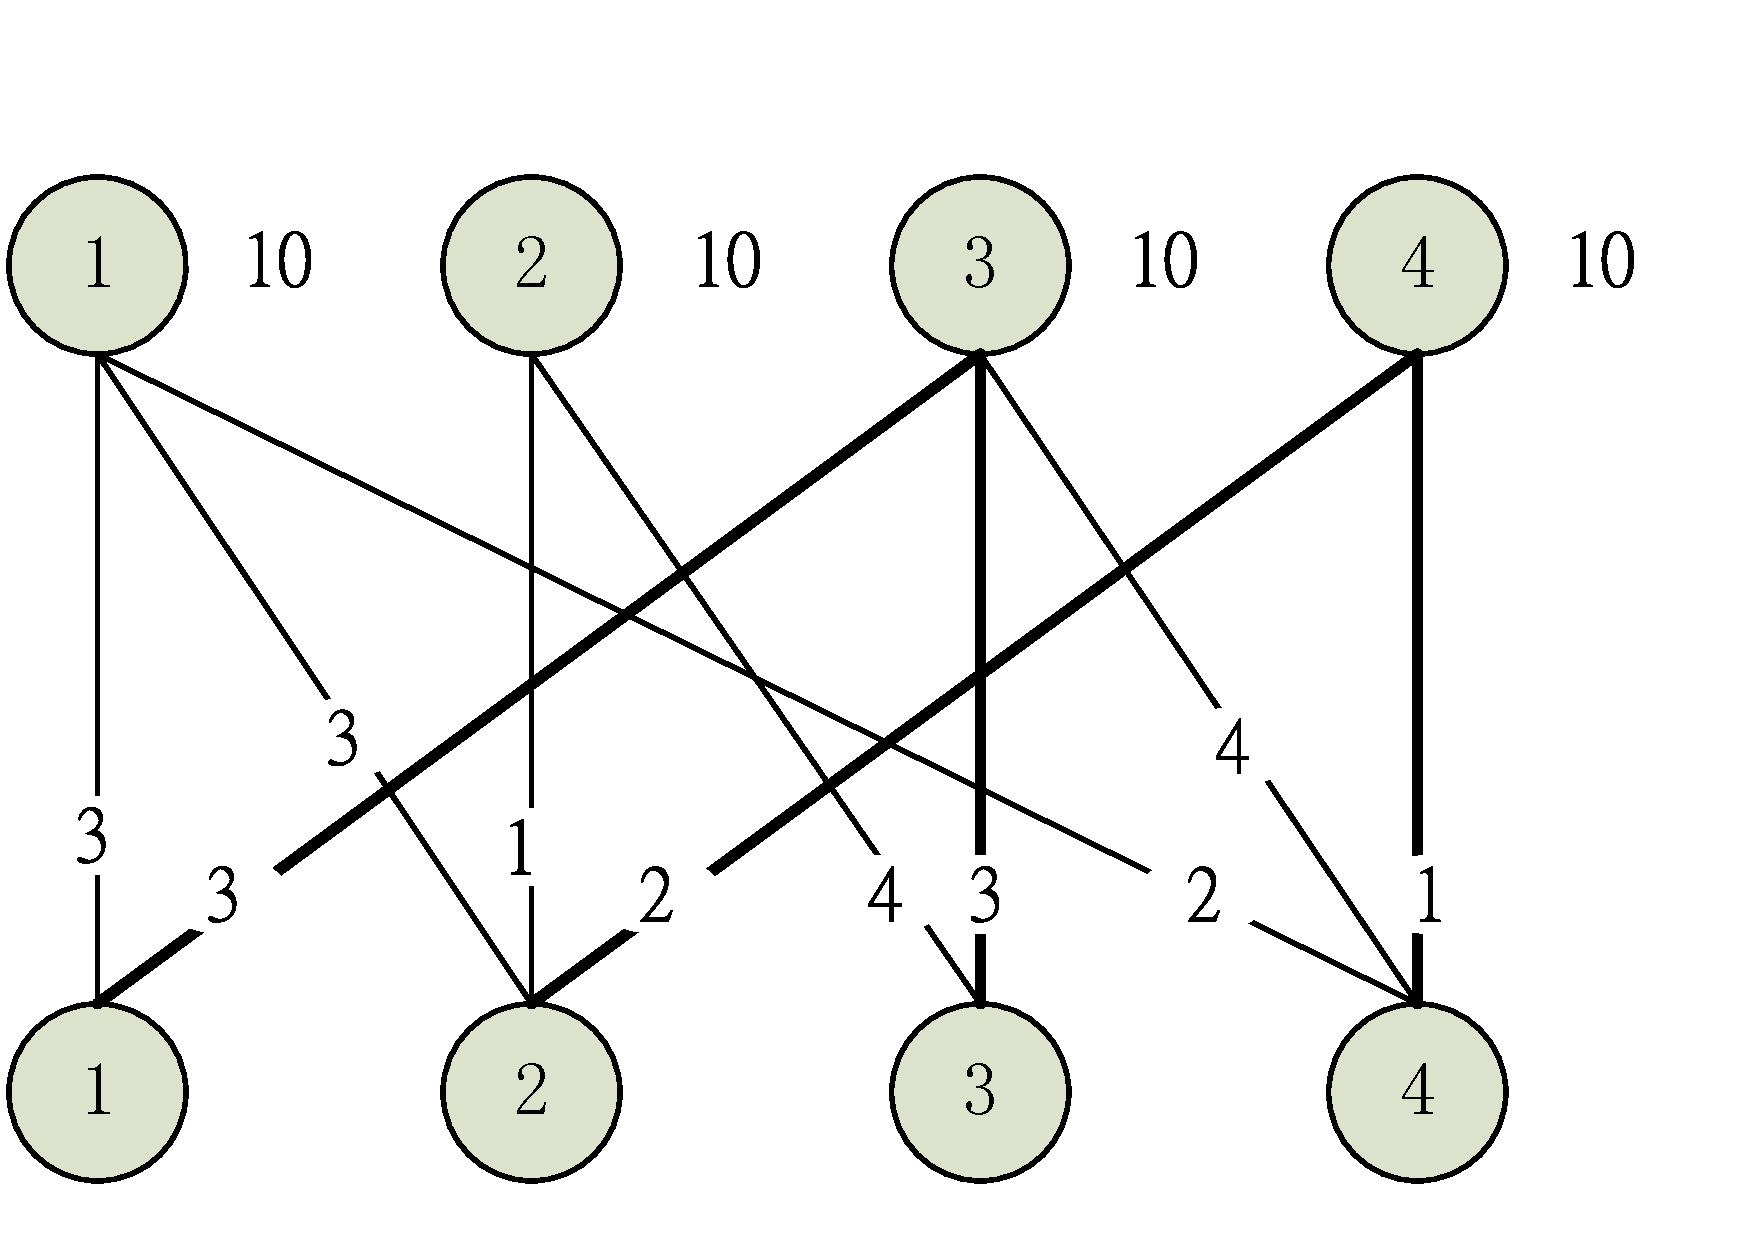
\includegraphics[width=0.5\textwidth]{figure-1.pdf}
      \caption{\label{figure:exampleUFL} UFL 博弈的一个例子}
      \vspace{-3mm}
      \end{figure}

      在图\ref{figure:exampleUFL}中所示的UFL博弈中,这里有四个设施和四个参与者。每一个设施有一个固定的启用成本10。在连接线上的数字代表从设施到参与者的运输成本。对于大联盟的一个最优解是开启设施3和4,并且画粗的连接线是最优路径。因此,大联盟所需要的成本是 10+10+3+3+2+1=29。

      在这个例子中,我们使用了两种 LP 求解方法,单纯形法和内点法,分别在 MATLAB 发行版本 2011a上计算LPB分配。
      表 \ref{table:UFLCA} 显示了在不同方法下的每一个参与者需要承担的成本。


      \begin{table}[H]
      \vspace{-2mm}
      \centering
      \tabcolsep=4pt
      \small
      \renewcommand\arraystretch{1.5}
      \caption{\label{table:UFLCA} 不同方法下的最优稳定UFL成本分配}
      \vglue5pt
      \begin{tabular}[!h]{c c c c c c c c c c c c c}
      \hline
      \multicolumn{1}{c}{方法}
      &\multicolumn{1}{c}{}
      &\multicolumn{1}{c}{参与者 1}
      &\multicolumn{1}{c}{}
      &\multicolumn{1}{c}{参与者 2}
      &\multicolumn{1}{c}{}
      &\multicolumn{1}{c}{参与者 3} &\multicolumn{1}{c}{}
      &\multicolumn{1}{c}{参与者 4}	&\multicolumn{1}{c}{}
      &\multicolumn{1}{c}{总共享成本}\\
      \hline
      单纯形法	& &5.00	& &6.50	& &8.50	& &6.50	&	&26.5	&\\
      内点法	& &6.58	& &6.50	& &8.50	& &4.92	&	&26.5	&\\
      LRB	& &6.87	& &6.50	& &8.50	& &4.63	&	&26.5	&\\
      \hline
      \end{tabular}
      \vspace{-3mm}
      \end{table}

      实例表明,LRB算法可以产生不同于一般LP方法的最优稳定成本分配。
      LRB解超出了两个LPB解的凸组合范围。
      这说明了LRB算法在提供替代成本分配方面的价值。

      为了研究LRB算法在一般设置下的能力,我们测试了由 \cite{Benchmark} 开发的30个无容量限制的设施位置基准实例,所有实例均有 $ M=N=100$。我们在一台Windows7 个人电脑上进行了所有的计算实验,该电脑的CPU型号为英特尔酷睿i7-2600,主频3.4GHz和内存为16G。所有算法均在Matlab 2011a版本中实现。
      在30个实例中,有22个实例的LRB解超出了两个LPB解的凸组合范围。
      同样,这显示了LRB算法在计算上寻找替代最优稳定成本分配方面的价值,即使在LPB成本分配显示为最优的情况下也是如此。

    \subsection{非线性有容量限制设施选址博弈}\label{section:NLCFL}
    在一个非线性有容量限制设施选址博弈(以下简称NLCFL博弈)中,存在一个和无容量限制设施选址博弈(以下简称UFL博弈)中定义类似的二部网络$G=(M,N,E)$。现每一个潜在的设施点$i \in M$有容量$Q_i$,每个客户$j \in N$有需求$q_j$。每一个客户只能由一个设施点提供服务。除了开业成本外,每一间设施$i$也有运营成本,该成本随着其服务客户数量的增加而增加。为了模拟经济中的规模效应,我们使用二次函数$\theta_i[h_i n_i - l_i\big(n_i \big)^2]$去衡量运营成本,其中$n_i$为设施$i$服务的顾客数量,$\theta_i$,$h_i$和$l_i$是特征函数的参数,该特征函数是凹函数,并且随着$n_i \in [0,n]$的增加而增加。
    在UFL博弈中,参与者仅仅局限于$N$中,与之不同的是,在NLCFL博弈中,参与者包括$M$中的设施参与者和$N$中的客户参与者。类似的参与者设置可以在装箱博弈中找到。我们的LRB算法也可以处理只有客户参与者参与的情况。然而,如果参与者中包括设施点参与者,并且特征函数为非线性的,我们则可以证明我们的LRB算法应用的广泛性。
    我们需要表3中的名词解释,去定义NLCFL博弈。
    \begin{table}[H]
    \vspace{-2mm}
    \centering
    \tabcolsep=7pt
    \small
    \renewcommand\arraystretch{1.5}
    \caption{\label{table:notations} 在NLCFL博弈中使用的新记号}
    \vglue5pt
    \begin{tabular}[!h]{c c}
    \hline
    \multicolumn{1}{c}{记号} &\multicolumn{1}{c}{含义}\\
    \cline{1-2}
    \multicolumn{1}{c}{$Q_i$} &\multicolumn{1}{l}{设施 $i$ 的容量, $\forall i \in M$, $Q_i \in \Z^+$.}\\
    \multicolumn{1}{c}{$q_j$} &\multicolumn{1}{l}{顾客 $j$ 的需求, $\forall j \in N$, $q_j \in \Z^+$.}\\
    \multicolumn{1}{c}{$s$} &\multicolumn{1}{l}{一个参与者联盟, $s = s_f \cup s_c$.}\\
    \multicolumn{1}{c}{$s_f$} &\multicolumn{1}{l}{联盟 $s$中的设施集合, $s_f \subseteq M$.}\\
    \multicolumn{1}{c}{$s_c$} &\multicolumn{1}{l}{联盟 $s$中的顾客集合, $s_c \subseteq N$.}\\
    \multicolumn{1}{c}{$\gamma^s$} &\multicolumn{1}{l}{示性向量 $\big[ \gamma^{s_f}_1,\gamma^{s_f}_2,...,\gamma^{s_f}_{m},\gamma^{s_c}_{1},\gamma^{s_c}_{2},...,\gamma^{s_c}_{n} \big]^T$, 如果 $i \in s_f$则$\gamma^{s_f}_i=1$ 否则 $\gamma^{s_f}_i=0$; }\\
    \multicolumn{1}{c}{} &\multicolumn{1}{l}{ 如果 $j \in s_c$ 则 $\gamma^{s_c}_j=1$ 否则有 $\gamma^{s_c}_j=0$,$\forall j \in N, s_f \subseteq M, s_c \subseteq N$.}\\
    \hline
    \end{tabular}
    \vspace{-3mm}
    \end{table}
    定义4. 一个NLCFL博弈$\big( M \cup N,c_{NLCFL} \big)$由$M \cup N$中的参与者定义,其中$M$是设施参与者集合,$N$是客户参与者集合,特征函数$c_{NLCFL}(s)$由NLP定义:
    \begin{equation}\label{eqn:cfobjnonlinear}
    c_{NLCFL}(s_f \cup s_c) = \min_{v,u}  \sum_{i \in M} f_iv_i + \sum_{i \in M}\sum_{j \in N} c_{ij}u_{ij} + \sum_{i \in M} \theta_i \big[ \sum_{j \in N}h_iu_{ij} - l_i \big(\sum_{j \in N}u_{ij}\big)^2 \big]
    \end{equation}
    \begin{equation}\label{eqn:concf1}
    s.t.~\sum_{i \in M} u_{ij} \geq \gamma_j^{s_c},~\forall j \in N,
    \end{equation}
    \begin{equation}\label{eqn:concf2}
    \sum_{j \in N}q_ju_{ij} - Q_iv_i \leq 0, ~\forall i \in M,
    \end{equation}
    \begin{equation}\label{eqn:concf4}
    v_i \leq \gamma_i^{s_f},~\forall i \in M,
    \end{equation}
    \begin{equation}\label{eqn:concf7}
     v_i,u_{ij}, \in \big\{0,1\big\},~\forall i \in M, j \in N.
    \end{equation}
    \end{definition}
    与$c_{UFL}(s)$相比,$c_{NLCFL}(s_f \cup s_c)$有一些新约束。 约束(26)代表设施的容量限制; 约束(27)确保只有当一个设施参与者在联盟中,相应的设施才可以用于服务客户。
    由于$c_{NLCFL}(s_f \cup s_c)$的目标函数在衡量设施运营成本的时候,具有非线性的部分,LPB算法不再适用计算成本分配。接下来,我们将说明LRB算法在NLCFL博弈上的应用。


      \subsubsection{NLCFL博弈中的LRB成本分配}\label{example-decompnlcfl}
      在NLCFL博弈中的特征函数$c_{NLCFL}(s_f \cup s_c)$中,通过增加一组新的约束
      \begin{equation}\label{eqn:CFLLRBR}
      u_{ij} \leq \gamma_i^{s_f}, ~u_{ij} \leq \gamma_j^{s_c},~\forall i \in M, j \in N,
      \end{equation},
      并将约束$\big\{\sum_{i \in M} u_{ij} \geq \gamma_j^{s_c}:\forall j \in N\big\}$乘上非负的拉格朗日乘子$\sigma$加入目标函数中,我们可以得到NLCFL博弈中的拉格朗日特征函数,
      \begin{eqnarray*}\label{eqn:LRCFnonlinear}
      \begin{aligned}
      \begin{split}
      c_{LR\_NLCFL}(s;\sigma) = \sum_{i \in M}f_iv_i + &\sum_{i \in M} \sum_{j \in N} \big(c_{ij} - \sigma_{j} + \theta_ih_i\big)u_{ij}
       - \sum_{i \in M} \theta_il_i \big( \sum_{j \in N}u_{ij}\big)^2 + \sum_{j \in N} \sigma_j \gamma_j^{s_c}\\
      s.t.~&\sum_{j \in N}u_{ij}q_j - Q_iv_i \leq 0,~\forall i \in M,\\
      ~~~~~~&~~u_{ij} \leq \gamma_i^{s_f},~\forall i \in M, j \in N,\\
      ~~~&~~~~~~v_i \leq \gamma_i^{s_f},~\forall i \in M,\\
      ~~~~~~&~~u_{ij} \leq \gamma_j^{s_c},~\forall i \in M, j \in N,\\
      v_i&, u_{ij} \in \{0,1\}, ~\forall i \in M, j \in N.
      \end{split}
      \end{aligned}
      \end{eqnarray*}
      与$c_{UFL}$中的约束(18)类似,约束(29)的作用是增强$c_{NLCFL}(s_f \cup s_c)$的下界。
      利用LRB算法,我们能把$c_{LR\_NLCFL}(\ \cdot\ ;\sigma)$分解成$c_{LR1\_NLCFL}(\ \cdot\ ;\sigma)$ 和 $c_{LR2\_NLCFL}(\ \cdot\ ;\sigma)$,即$c_{LR\_NLCFL}(s_f \cup s_c;\sigma) = c_{LR1\_NLCFL}(s_f \cup s_c;\sigma) + c_{LR2\_NLCFL}(s_f \cup s_c;\sigma)$, for all $s_f \subseteq M$ and $s_c \subseteq N$
      并且定义NLCFL sub-game 1 $\big(M \cup N;c_{LR1\_NLCFL}(\ \cdot\ ;\sigma)\big)$ 和 NLCFL sub-game 2 $\big(M \cup N;c_{LR2\_NLCFL}(\ \cdot\ ;\sigma)\big)$。
      对于NLCFL subgame 1,特征函数是
      \begin{eqnarray}\label{eqn:ncgcf}
      \begin{aligned}
      \begin{split}
      c_{LR1\_NLCFL}(s_f \cup s_c,\sigma) = \sum_{j \in N} \sigma_j\gamma_j^{s_c}.
      \end{split}
      \end{aligned}
      \end{eqnarray}
      根据引理1,我们可以得出博弈$\big(M \cup N, c_{LR1\_NLCFL}(\ \cdot \ ;\sigma)\big)$的核心成本分配,其中每个客户参与者$j \in N$都被分配一个成本,准确等于服务她的拉格朗日对偶价格,没有设施参与者被分配任何费用,因为他们不需要服务。成本分配为$\alpha_{LR1\_NLCFL}^{\sigma}(j) = \sigma_j$ for all $j \in N$, 和 $\alpha_{LR1\_NLCFL}^{\sigma}(i) = 0$ for all $i \in M$。
      对于NLCFL 子博弈2,特征函数为
      \begin{eqnarray*}
      \begin{aligned}
      \begin{split}
      c_{LR2\_NLCFL}(s_f \cup s_c;\sigma) = \min_{v,u}& \sum_{i \in M} f_iv_i + \sum_{i \in M}\sum_{j \in N} \big(c_{ij} - \sigma_j + \theta_ih_i\big) u_{ij} - \sum_{i \in M} \theta_il_i \Bigl( \sum_{j \in N}u_{ij}\Bigr)^2\\
      s.t.~&\sum_{j \in N}u_{ij}q_j - Q_iv_i \leq 0,~\forall i \in M,\\
      ~~~~&~~u_{ij} \leq \gamma_i^{s_f},~\forall i \in M, j \in N,\\
      &~~~~~~v_i \leq \gamma_i^{s_f},~\forall i \in M,\\
      ~~~~&~~u_{ij} \leq \gamma_j^{s_c},~\forall i \in M, j \in N,\\
      v_i&, u_{ij} \in \{0,1\}, ~\forall i \in M, j \in N.
      \end{split}
      \end{aligned}
      \end{eqnarray*}
      为了解决$c_{LR2\_NLCFL}(s_f \cup s_c;\sigma)$,我们能够依照设施来分离它,$c_{LR2\_NLCFL}(s_f \cup s_c;\sigma) = \sum_{i \in s_f} \psi^i(s_c;\sigma)$,其中对于每一个$i \in s_f$,
      \begin{eqnarray}\label{eqn:psi}
      \begin{aligned}
      \begin{split}
      \psi^i(s_c;\sigma) = \min_{v_i,u_{ij}} f_iv_i + \sum_{j \in s_c} \big(c_{ij} - \sigma_j + \theta_ih_i\big)& u_{ij} - \theta_il_i \Bigl( \sum_{j \in s_c}u_{ij}\Bigr)^2\\
      s.t. ~~ \sum_{j \in s_c}q_ju_{ij} - Q_iv_i \leq 0,&\\
      v_i,u_{ij} \in \big\{0,1\big\},~\forall j \in s_c&.
      \end{split}
      \end{aligned}
      \end{eqnarray}
      可以看出,对于每个问题$\psi^i(s_c;\sigma)$都符合背包问题的变体,该背包问题的目标函数是最小化非线性总值,其中$Q_i$是背包容量,$s_c$是物品的集合,每个物品$j\in s_c$都具有权重$q_j$和值$(c_{ij}-\sigma_j+\theta_ih_i)$。除装在背包中的物品的总价值外,参与者可以获得一个额外的价值$-\theta_il_i \Bigl( \sum_{j \in s_c}u_{ij}\Bigr)^2$,它是装在背包中的物品数量的二次方。当所有权重$q_j$都是整数,我们可以用动态规划在伪多项式时间$O(Q_in^2)$内解决$\psi^i(s_c;\sigma)$。具体来说,我们将$F^{s_c}_i(j,k,q)$定义为$\sum_{j'\in s_c,j'\leq j}(c_{ij'}-\sigma_{j'}+\theta_ih_i)u_{ij'}$的最小值,以至于$\sum_{j'\in s_c,j'\leq j}u_{ij'}=k$并且$\sum_{j'\in s_c,j'\leq j}q_{j'}u_{ij'}\leq q$。换句话说,$F^{s_c}_i(j,k,q)$中的自变量包括从$\{1,2,\cdots,j\}$中取出的$k$个值以及容量$q$,其代表着装入背包中物品的最小价值。
      动态规划递归方程如下:
      \begin{eqnarray*}
      \begin{aligned}
      \begin{split}
      F^{s_c}_i(j,k,q)=\left\{
      \begin{array}{ll}
      F^{s_c}_i(j,k,q), & \mbox{ if } j\not\in s_c,
      \\[3mm]
      \min\big\{F^{s_c}_i(j-1,k,q),F^{s_c}_i(j-1,k-1,q-q_j) \big\}, & \mbox{ if } j\in s_c,
      \end{array}\right.
      \end{split}
      \end{aligned}
      \end{eqnarray*}
      其初始条件为:
      $F^{s_c}_i(0,0,q)=0$ for  $q\geq 0$
      其边界条件为:
      $F^{s_c}_i(j,k,q)=+\infty$ for $q<0$
      从而,
      $\psi_i(s_c;\sigma)$可以通过$\psi_i(s_c;\sigma) = \min_{k\leq |s_c|}\bigl\{ 0, f_i+F^{s_c}_i(n,k,Q_i)-\theta_i l_i k^2\bigr\}$找到,并且我们有$c_{LR2\_NLCFL}(s_f \cup s_c;\sigma) = \sum_{i \in s_f} \psi_i(s_c;\sigma)$。
      现在,我们已准备通过CGB算法计算NLCFL 子博弈 2的最佳稳定的成本分配$\alpha_{LR2\_NLCFL}^{\sigma}$,此处我们需要解决一个定价问题。在这种特殊情况下,定价问题是用最小的降低成本找到一个联盟(或列)$s=s_f \cup s_c$,此处每个$s = s_f \cup s_c$的降低成本为
      \begin{eqnarray}\label{eqn:pricing1nlcfl}
      \begin{aligned}
      \begin{split}
      \min_{v,u}  \sum_{i \in s_f} f_i v_i + \sum_{i \in s_f}\sum_{j \in s_c} &\big(c_{ij} - \sigma_j + \theta_ih_i\big)u_{ij} - \sum_{i \in s_f} \theta_il_i \Bigl( \sum_{j \in s_c}u_{ij}\Bigr)^2 - \sum_{k \in M \cup N} \gamma^s_k \pi_k^*\\
      &s.t. ~~\sum_{j \in s_c}q_ju_{ij} \leq Q_iv_i, ~\forall i \in s_f,\\
      &v_i, u_{ij} \in \big\{0,1\big\},~\forall i \in s_f, j \in s_c,
      \end{split}
      \end{aligned}
      \end{eqnarray}
      其中,$\pi^*$是NLCFL 子博弈 2的相应大规模问题的最佳对偶。
      对于每个给定的$s=s_f\cup s_c$,我们可以直接获得(32)的最佳目标值,它等于$\sum_{i\in s_f}\psi^{i}(s_c;\sigma)-\sum_{k \in M \cup N} \gamma^s_k \pi_k^*$,其中对于每个$\psi^{i}(s_c;\sigma)$,如前所示,可以通过动态规划来计算。然而,由于指数数量的联盟,用枚举法去寻找一个最负减少成本的列$s$,这在计算上是难以处理的。因此,我们通过考虑以下两种情形,尝试在一开始定义一个最负减少成本的列$\bar{s}$:
      情形1.至少存在一个k使得$\pi^*_k>0$。在这种情况下,可以通过包括$k$ with $\pi^*_k>0$,$k\in M \cup N$来定义联盟$\bar s$,对于$\bar s$的降低成本是负的,因为通过让所有的$u$ 和 $v$都趋向于0,$\bar s$至多为$-\sum_{k\in M\cup N} \max\{0, \pi^*_k\}$。
      情形2.对于所有$k\in M\cup N$,  $\pi^*_k \leq 0$。这种情况更加的复杂。为了有效地找到一个负成本的联盟$\bar s = \bar{s}_f \cup \bar{s}_c$,我们可以考虑以下的ILP,其中二进制变量$v_i$和$\gamma_j$分别表示$\bar{s}$是否包括设施点参与者$i$和客户点参与者$j$,这里$f'_i = f_i - \pi_i^*$, $c'_{ij} = c_{ij}-\sigma_j + \theta_ih_i$, $l'_i = \theta_il_i$ 并且 $\pi'_j = -\pi_j^*$。
      \begin{eqnarray}\label{eqn:pricing2nonlinear}
      \begin{aligned}
      \begin{split}
      \min_{v;u;\gamma} R(v,u,\gamma) = \min_{v,u} &\sum_{i \in M} f'_i v_i + \sum_{i \in M}\sum_{j \in N} c'_{ij}u_{ij} - \sum_{i \in M} l'_i \big(\sum_{j \in N}u_{ij}\big)^2+ \sum_{j \in N} \gamma_j \pi'_j\\
      s.t.&~~\sum_{j \in N}q_ju_{ij} \leq Q_iv_i, ~\forall i \in M,\\
      &u_{ij} \leq \gamma_j,~\forall i \in M, j \in N,\\
      v_i, u_{ij}&, \gamma_j \in \big\{0,1\big\},~\forall i \in M, j \in N,
      \end{split}
      \end{aligned}
      \end{eqnarray}
      因此,可以看出负的目标值得ILP的可行解,是和负的减少成本的联盟$\bar{s} =  \bar{s}_f \cup \bar{s}_c$一一对应的。而且,通过利用以下属性,这样的联盟$\bar{s}$可以有效获得。\\
      \textbf{引理5}. 对于(33),在不改变最佳目标值的情况下,我们可以通过以下步骤将一些变量依次固定为零:
      (1)对于每个$(i,j)\in M\times N$,如果$c'_{ij} - l'_i\big[n_i^2 - (n_i-1)^2\big] > 0$,则$u_{ij}=0$,其中$n_i$是集合$\{c'_{ij} < \infty: \forall j \in N\}$中元素的数量。之后,设置$c'_{ij}=\infty$。
      (2)对于每个$j\in N$,如果$\pi'_j+\sum_{i\in M}\min\{c'_{ij}- l'_i\big[n_i^2 - (n_i-1)^2\big],0\} \geq 0$,则$\gamma_j=0$, $ u_{ij}=0$,  $\forall i\in M$.
      (3)对于每个$i\in M$,求解非线性背包问题类似于(31),其中$Q_i$是背包容量,$N$是物品集合,每个物品$j\in N$具有权重$q_j$和值$c'_{ij}$。让$\omega^i$是这个背包问题的最优目标函数值。如果$\omega^{i} + f'_{i} \geq 0$,则$v_i=0$,$u_{ij}=0$,for all $j\in N$。
      证明:首先,如果存在一对索引$(i,j)$,使得ILP(33)的可行解中的$u_{ij} = 1$ 和 $c'_{ij} - l'_i\big[n_i^2 - (n_i-1)^2\big] > 0$,我们可以直接设置$u_{ij} = 0$,并推导出另一个可行解,在此基础上,目标函数值将至少减少$c'_{ij} - l'_i\big[n_i^2 - (n_i-1)^2\big]$。
      第二,如果存在客户 $j$,使得ILP(33)的可行解 $\gamma_j = 1$,$\pi'_j+\sum_{i\in M}\min\{c'_{ij}- l'_i\big[n_i^2 - (n_i-1)^2\big],0\} \geq 0$ in a feasible solution of ILP $(\ref{eqn:pricing2nonlinear})$, 则对于所有的$i \in M$设置$\gamma_j = 0$,$u_{ij} = 0$,这将推导出另一个可行解,此处的目标函数值将至少减少$\pi'_j+\sum_{i\in M}\min\{c'_{ij}- l'_i\big[n_i^2 - (n_i-1)^2\big],0\}$。
      第三,如果存在设施$i$,使得ILP(33)的可行解中,$v_i = 1$,$\omega^{i} + f'_{i} \geq 0$,则对于所有的$j \in N$,通过设置$v_i = 0$,$u_{ij} = 0$的解也是可行的,并且目标函数值将减少至少$\omega^{i} + f'_{i}$。
      上述引理只想说明,做出上述改动并不能增加$\min_{v;u;\gamma} R(v,u,\gamma)$。虽然理论上没有确保多项式时间复杂度,但是引理5中的步骤确实可以大大减少求解(33)时的问题规模。
      在得出NLCFL 子博弈 1 and 2最优稳定成本分配$\alpha_{LR1\_NLCFL}^{\sigma}$和$\alpha_{LR2\_NLCFL}^{\sigma}$之后,我们可以根据定理1计算NLFCL博弈的稳定成本分配$\alpha_{LR\_NLCFL}^{\sigma} = \alpha_{LR1\_NLCFL}^{\sigma} + \alpha_{LR2\_NLCFL}^{\sigma}$。更重要的是,通过定理2,如果$\sigma^*$是最优的拉格朗日乘子,并且$\big(M \cup N;c_{LR2\_NLCFL}(\ \cdot\ ;\sigma^*)\big)$有一个非空的核心,则相应的LRB成本分配数值$\sum_{k \in M\cup N}\alpha^{\sigma^*}_{LR\_NLCFL}(k)$都是等于拉格朗日松弛下界$c_{LR\_NLCFL}(M \cup N;\sigma^*)$。

      \subsubsection{非线性有容量限制设施选址博弈的计算结果}\label{sec:nlcflcomputation}
      为了进行数值实验,我们用20个由Beresnev等人(2006)开发的单一资源设施位置基准实例。每个实例均有一个二部网络$G=(M,N,E)$,其中$m=n=100$,并且对于所有的$i \in M$,$f_i=100$。对于每个例子,都有三个容量级别10,20和30。另外,我们使用$h_1 = h_2 = ... = h_m = n^2$, $l_1 = l_2= ... = l_m = 1$, $\theta_1 = \theta_2 = ... = \theta_m=\theta$去衡量运营成本,这里$\theta$表示运营成本的相对权重。当通过次梯度法去解决拉格朗日对偶问题时,我们设置的最大迭代次数是2500。
      为了显示LRB成本分配的有效性,理想情况下,我们需要比较总共享成本和大联盟成本$c_{NLCFL}(M \cup N)$。然而,大联盟的成本只能在$\theta=\textbf{0}$的基准实例数据集中可以利用。因此,对于一般比较,我们需要通过启发式解去替换中心最优解,该启发式解叫做最好的被发现的中心解(BFCS),这被定义为下列两个可行的解决方案中的较好的那个。第一个可行解是$\theta = \textbf{0}$ 的NLCFL问题的初始基准实例的最优解,Bachrach等人(2009年)研究过该解。第二个可行解可由$c_{LR2\_NLCFL}(M \cup N;\sigma)$的最优解推导出来。提醒一下,这种最优解对于中心化问题$c_{NLCFL}(M \cup N)$可能是不可行的,因为有些客户可能没有被服务。如果是这样,那就是对于给定的不可行解得出一个可行解,我们可以继续进行如下。对于每个未得到服务的客户,我们选择一个已开办的设施点,其有足够的剩余容量,以及服务这个客户的最小运输成本;如果没有这样的设施,我们就开辟拥有最小运输成本的新的可行性设施去服务这个客户。
      表4展示了在20个实例中,设施容量均一致等于10,20,30的情形下,LRB成本分配算法应用的效果和计算效率。
      \begin{table}[H]
      \vspace{-2mm}
      \centering
      \tabcolsep=6pt
      \small
      \renewcommand\arraystretch{1.4}
      \caption{\label{table:LRBNSG} LRB 对于NLCFL博弈的成本分配算法表现}
      \vglue5pt
      \begin{tabular}[!h]{c c c c c c c c c c c c c c}
      \hline
      \multirow{2}{*}{容量} &\multirow{2}{*}{$\theta$} &\multicolumn{1}{c}{} & \multicolumn{3}{c}{LRCA / BFCS (\%)} &\multicolumn{1}{c}{} & \multicolumn{3}{c}{LRCA / LRB(\%)}  &\multicolumn{1}{c}{} & \multicolumn{3}{c}{总时间 (s)}\\
      \cline{4-6}
      \cline{8-10}
      \cline{12-14}
      & & & Average & Max &Min	& & Average & Max &Min & & Average & Max &Min\\
      \hline
      \multirow{5}{*}{$Q=10$}
      &0  &  &98.79	&99.12	&98.33	&	&100	&100	&100	&	&--	&--	&--\\

      &0.01  &  &99.64	&99.70	&99.55	&	&100	&100	&100	&	&5683	&6838	&4987\\

      &0.1  &  &99.87	&99.89	&99.78	&	&100	&100	&100	&	&5690	&6834	&4980\\

      &0.5  &  &99.90	&99.92	&99.87	&	&100	&100	&100	&	&5742	&6814	&5036\\

      &1  &  &99.91	&99.95	&99.89	&	&100	&100	&100	&	&5822	&6983	&4764\\
      \hline
      \multirow{5}{*}{$Q=20$}
      &0  &  &98.32	&99.30	&97.66	&	&100	&100	&99.95	&	&--	&--	&--\\

      &0.01  &  &99.61	&99.76	&99.48	&	&100	&100	&100	&	&9925	&10478	&9485\\

      &0.1  &  &99.83	&99.85	&99.82	&	&100	&100	&100	&	&9835	&10458	&9322\\

      &0.5  &  &99.85	&99.88	&99.84	&	&100	&100	&99.99	&	&9825	&10487	&9315\\

      &1  &  &99.89	&99.92	&99.87	&	&100	&100	&100	&	&9973	&11154	&9812\\
      \hline
      \multirow{5}{*}{$Q=30$}
      &0  &  &95.25	&96.95	&93.93	&	&100	&100	&100	&	&--	&--	&--\\

      &0.01  &  &99.02	&99.15	&98.82	&	&100	&100	&99.99	&	&11686	&12831	&10410\\

      &0.1  &  &99.72	&99.77	&99.63	&	&99.99	&100	&99.95	&	&11755	&12816	&10421\\

      &0.5  &  &99.81	&99.87	&99.78	&	&100	&100	&100	&	&11485	&13064	&10277\\

      &1  &  &99.88	&99.92	&99.86	&	&100	&100	&100	&	&12621	&14371	&11955\\
      \hline
      \end{tabular}
      \vspace{-3mm}
      \end{table}
      在表4中,“LRCA”表示在不同的$\sigma$下,找到的最佳LRB成本分配值$\sum_{k \in M \cup N}\alpha_{LR\_NLCFL}^{\sigma}(k)$,而“LRB”代表用次梯度法求得的最好的拉格朗日下界$c_{LR\_NLCFL}(M \cup N; \sigma^*)$。对于每个容量,我们列出了在不同的$\theta$值下的计算结果。从列“LRCA / BFCS”可以看出,对于所有检查的实例,我们的LRB成本分配算法可以产生稳定的成本分配,至少达到BFCS的$93.93\%$。当$\theta$增加,以至于设施运营成本增加了更多的权重,我们的LRB成本分配可以分享BFCS超过$99\%$。这些发现表明了LRB成本分配的高品质。而且,尽管NLCFL子博弈2通常没有次模性,列“LRCA / LRB”表明几乎每个NLCFL子博弈2都有一个非空的核心。这表明甚至在定理2的条件(2)不满足的情况下,LRB成本分配仍有很大可能达到拉格朗日下界。至于时间效率,我们可以看到计算时间趋于随着$Q$ 和 $\theta$的增加而增加。在所有情况下,最长的计算时间大约是四个小时。
      对于$\theta=\textbf{0}$的情形,NLCFL博弈在其特征函数中没有非线性项,我们通过展示在表5中的成本分配值和基准实例中的大联盟成本之比,即比较LPB和LRB的成本分配。这里,是LPB和LRB成本分配是基于在约束(29)中提到的相同的特征函数$c_{NLCFL}(s_f \cup s_c)$ 的ILP算式计算的。
      \begin{table}[H]
      \vspace{-2mm}
      \centering
      \tabcolsep=14pt
      \small
      \renewcommand\arraystretch{1.5}
      \caption{\label{table:LRBLPBSG} 当 $\theta = \textbf{0}$ 时,LPB vs. LRB 对于 NLCFL 博弈的成本分配结果 (in \%)}
      \vglue5pt
      \begin{tabular}[!h]{c c c c c c c c c c}
      \hline
      \multirow{2}{*}{容量} & \multicolumn{5}{c}{Average}	&\multicolumn{1}{c}{} & \multicolumn{2}{c}{LRCA $-$ LPCA}\\
      \cline{2-6}
      \cline{8-9}
      & LPCA & LRB & LRCA	& LRB$'$ & LRCA$'$	& &Max	&Min\\
      \hline
      10    &97.15	&98.79	&98.79	&98.79	&98.79	&	&2.38	&1.00\\

      20    &97.20	&98.32	&98.31	&98.29	&98.25	&	&1.51	&0.88\\

      30    &94.70	&95.25	&95.25	&95.21	&95.21	&	&0.75	&0.38\\

      40    &94.11	&94.25	&94.25	&94.25	&94.25	&	&0.28	&0.07\\

      50    &93.87	&93.88	&93.88	&93.88	&93.88	&	&0.04	&-0.02\\
      \hline
      \end{tabular}
      \vspace{-3mm}
      \end{table}
      为了研究约束$(\ref{eqn:CFLLRBR})$的影响,我们用新的拉格朗日下界LRB$'$ 和新的LRB成本分配值LRCA$'$去比较LRB和LRCA,其中LRB$'$和LRCA$'$可从约束$(\ref{eqn:CFLLRBR})$被松弛后的修订特征函数$c_{LR_NLCFL}(s;\sigma)$中获得。而且,因为LPB的成本分配值和LP下界是相等的,他们都被放在表\ref{table:LRBLPBSG}的“LPCA”栏中,从表格中,我们可以观察到以下结论。
      首先,平均来看,如前两个 “平均值”下的列所示,拉格朗日下界比LP下界更紧。这意味着LRB成本分配相对LPB成本分配有潜在的优势。另外,如``LRCA $-$ LPCA''下的列所示,平均而言,LRB成本分配是确实优于LPB,特别是对于容量较小的案例。
      其次,如``LRB, LRCA, LRB$'$, LRCA$'$"栏中所示,“将约束(29)添加到$c_{NLCFL}(s_f \cup s_c)$ 确实可以提高拉格朗日下界和LRB成本分配值。另外,通过比较列``LPCA" 和 ``LRCA$'$",我们发现,平均来看,即使没有额外的限制条件, LRB成本分配结果平均仍然优于LPB。这进一步意味着我们LRB算法的竞争力。
      我们接下来研究NLCFL博弈中LRB算法的收敛性。这不是UFL博弈的的情形。在一个UFL博弈中,只要用次梯度法解拉格朗日对偶问题收敛于$\sigma^*$,因为UFL子博弈2具有非空的核心,定理2确保了符合$\sigma^*$的稳定成本分配的最优性。然而,NLCFL子博弈2可能有一个空核,这就暗示拉格朗日下界和能被分配的总成本之间可能存在的差距。虽然我们可能认为一个一般化的趋势是更好的拉格朗日下界将会带来更好的成本分配,但是当拉格朗日下界增加时,并不能保证成本分配的值严格增加。
      为了检验这一点,我们将算法1应用于NLCFL博弈上,此实例中,$\theta=\textbf{0}$,并且通过使用不同的拉格朗日乘子集合$\Lambda$,比较LRB成本分配。表6展示了当$\Lambda$ 从一个基准集 $\Lambda_2$ 变到另一个集 $\Lambda_1$,LRB成本分配分别得到改善,倒退和没有发生改变的实例数。每个$\sigma^{i}$代表在算法1的步骤1用次梯度法的第$i$次迭代中,找到的最好的拉格朗日乘子。结果显示,随着拉格朗日下界的改善,成本分配可能会变得更加糟糕,尽管在以后的迭代中,变坏的可能性非常小。例如,在一百个实例中,当$\Lambda$ 选择的是 $\{\sigma^{2500}\}$ 而不是 $\{\sigma^{500},\sigma^{800},\sigma^{1000},\sigma^{1500},\sigma^{2000}\}$时,有七个实例的LRB成本分配会下降。这个发现印证了在算法1中使用多个拉格朗日乘数的必要性。
      \begin{table}[H]
      \vspace{-2mm}
      \centering
      \tabcolsep=9pt
      \small
      \renewcommand\arraystretch{1.5}
      \caption{\label{table:CFLIterations}
      从不同的$\Lambda$拉格朗日乘子集合生成的LRB成本分配的比较}
      \vglue5pt
      \begin{tabular}[!h]{c c c c c}
      \hline
      \multicolumn{2}{c}{Pairs of $\Lambda$ sets} &\multirow{2}{*}{\# of Improved}	&\multirow{2}{*}{\# of Declined}	&\multirow{2}{*}{\# of Unchanged}\\
      \cline{1-2}
      $\Lambda_1$ &$\Lambda_2$ (as baseline) &\\
      \hline
      $\big\{\sigma^{800}\big\}$  &$\big\{\sigma^{500}\big\}$   &95	&4	&1\\

      $\big\{\sigma^{1000}\big\}$ &$\big\{\sigma^{500}, \sigma^{800}\big\}$     &51	&6	&43\\

      $\big\{\sigma^{1500}\big\}$ &$\big\{\sigma^{500},\sigma^{800},\sigma^{1000}\big\}$     &24	&6	&70\\

      $\big\{\sigma^{2000}\big\}$ &$\big\{\sigma^{500},\sigma^{800},\sigma^{1000},\sigma^{1500}\big\}$     &1	&6	&93\\

      $\big\{\sigma^{2500}\big\}$ &$\big\{\sigma^{500},\sigma^{800},\sigma^{1000},\sigma^{1500},\sigma^{2000}\big\}$     &0	&7	&93\\
      \hline
      \end{tabular}
      \vspace{-5mm}
      \end{table}
      总之,从计算实验来看,我们可以得出结论,LRB算法在解决NLCFL博弈的OCAP时,是高效的。

\section{结论}\label{sec:conclude}
本文的研究重点是核心可能为空的合作博弈。我们提出一个通用算法来计算得到一个最优的稳定费用分摊方案,使其在满足联盟的稳定性的条件下尽可能地覆盖大联盟的成本。在以往地研究中,这类问题主要通过LP松弛和对偶理论求解。我们采用与其不同的拉格朗日松弛理论求解。该方法的拉格朗日松弛下界不仅比现行松弛下界更具有竞争力,还打破了依赖于可分配约束和线性目标函数的局限。在两种代表典型的设施选址博弈应用该算法,结果表明该算法能够为这些博弈提供近乎最优的费用分摊方案,优于现有的LPB算法。

\bibliographystyle{ijocv081}
\bibliography{ComputingGoodCAforORGames}

\newpage

\end{document}
